\documentclass[bsc]{abdnthesis}

%% For citations, I would recommend natbib for its                          
%% flexibility, particularly when named citation styles are used, but                
%% it also has useful features for plain and those of that ilk.                      
%% The natbib package gives you the following definitons                             
%% that extend the simple \cite:                                                     
%   \citet{key} ==>>                Jones et al. (1990)                              
%   \citet*{key} ==>>               Jones, Baker, and Smith (1990)                   
%   \citep{key} ==>>                (Jones et al., 1990)                             
%   \citep*{key} ==>>               (Jones, Baker, and Smith, 1990)                  
%   \citep[chap. 2]{key} ==>>       (Jones et al., 1990, chap. 2)                    
%   \citep[e.g.][]{key} ==>>        (e.g. Jones et al., 1990)                        
%   \citep[e.g.][p. 32]{key} ==>>   (e.g. Jones et al., p. 32)                       
%   \citeauthor{key} ==>>           Jones et al.                                     
%   \citeauthor*{key} ==>>          Jones, Baker, and Smith                          
%   \citeyear{key} ==>>             1990                                             

\usepackage{float}
\usepackage{xcolor}
\usepackage{wrapfig}
\usepackage{minted, color, pdflscape, caption, tabularx, appendix, tocvsec2}
\usepackage{subcaption}
\usepackage{amsmath,amssymb,amsthm}
\usepackage{thmtools}
\usepackage[hidelinks, breaklinks]{hyperref}
\usepackage{cleveref}
\usepackage[round,colon,authoryear]{natbib}
\setlength{\bibsep}{0pt}
\usepackage{csquotes}
\usepackage[ruled,vlined,linesnumbered]{algorithm2e}

\usepackage{microtype}
\DisableLigatures[?,!]{encoding=T1}

\usepackage{etoolbox}
\PassOptionsToPackage{hyphens}{url}

\defcitealias{TestCoverageMediaWiki}{MediaWiki test coverage}
\defcitealias{ExtensionTestCoverageMediaWiki}{MediaWiki extension test coverage}
\defcitealias{mediawiki:GitReviewers}{Git Reviewers list}
\defcitealias{mediawiki:developersmaintainers}{Code maintainers list}
\defcitealias{GitExtensionsList}{list of extensions on MediaWiki's git repositories}

\newcommand{\rcnote}[1]{\noindent \textcolor{red}{Rafael: {#1}}}

\newcommand{\williamnote}[1]{\noindent \textcolor{blue}{William (self-note): {#1}}}

\newcommand{\williamnoteforrafael}[1]{\noindent \textcolor{blue}{William (for Rafael): {#1}}}

\newcommand{\citepmediawiki}[1]{(MediaWiki contributors, \citeyear{#1})}

\usepackage[T1]{fontenc}
\bibliographystyle{plainnat}

\title{Automatic code reviewer recommendations in the open-source project MediaWiki}
\author{William Brown}
% IMO this is a bit silly, but some like to include these. To remove,
% delete this declaration and remove the option from the
% \documentclass definition above.
%\qualifications{PhD, Computer Science, University College London, 1997\\%            
%BEng (Hons.) Electrical and Electronic Engineering, The University of Wales, Swansea, 1992}
\school{Department of Computing Science}

%%%% In the final submission of a thesis, this should only be the year
%%%% of submission.  However, it is useful to use \date{\today} for drafts so that
%%%% they don't get mixed up.
    
\date{2023}



%% It is useful to split the document up as chapters and include
%% them.  LaTeX will sort out all the numbering and cross-referencing
%% for you --- if you run it enough times!

%% If you want to include only a couple of chapters then use the
%% \includeonly{} command with a list of the file/chapter names that
%% you wish to include.  NB, this must be in the preamble.

% \includeonly{introduction,faq}

\def\sfthing#1#2{\def#1{\mbox{{\small\normalfont\sffamily #2}}}}

\sfthing{\PP}{P}
\sfthing{\FF}{F}

\def\UrlBreaks{\do\/\do-}
\def\UrlBigBreaks{\do\/\do-}

%% This will make sure that all cross-references are correct (including
%% references to those file not included) but will produce a dvi
%% file with only those files/chapters you specify included.

\begin{document}

%%%% Create the title page and standard declaration.

\maketitle
\makedeclaration

%%%% Then the abstract and acknowledgements

\begin{abstract}
\rcnote{You want the abstract to cover the entire page or be close to it (but do not go over one page).}

  Code review is a critical part of software development which catches bugs and improves the quality of the code. However, identifying appropriate reviewers in a large project with many potential reviewers is a challenge. \rcnote{Talk more about the challenges and why it can be so challenging.}
  
  In this report we implement a rule based and neural network based recommender implementations to automatically recommend reviewers for changes in the open-source project ``MediaWiki''. To make these recommendations a large dataset of items including code review votes, comments and code history is collected and applied to the implementations. \rcnote{Talk more about the approach here.}
  
  The evaluation results suggest that ... %We finally discuss the implications of the evaluation and detail future research opportunities created by this report.
\end{abstract}

\begin{acknowledgements}
\begingroup
\let\clearpage\relax
  \include{"other/acknowledgements"}
  \endgroup
\end{acknowledgements}

%%%% It should have a table of contents, but delete the other two as
%%%% necessary.

\tableofcontents
\listoftables
\listoffigures

% \clearpage
% \begingroup
% \let\clearpage\relax
\include{"main/introduction"}
\include{"main/background-related-work"}
\include{"main/requirements"}
\include{"main/implementation"}
\include{"main/evaluation"}
\include{"main/conclusion"}
% \endgroup

\bibliography{mybib}

\appendix
\settocdepth{chapter}
% \include{proof}
\chapter{Technical Manual\label{appendix:technical-manual}}
\chapter{User Manual\label{appendix:user-manual}}
\chapter{Detailed results\label{appendix:detailed-results}}

\let\svaddcontentsline\addcontentsline
\renewcommand\addcontentsline[3]{%
  \edef\qtest{#1}%
  \def\qmatch{lof}%
  \ifx\qmatch\qtest\else%
    \def\qmatch{lot}%
    \ifx\qmatch\qtest\else%
      \svaddcontentsline{#1}{#2}{#3}%
  \fi\fi%
}

In this Appendix the results are shown in full for the repositories that were used for evaluation. The results for the confusion matrix are not detailed here as doing so in full would add too many pages. However, all these results are available at the GitHub repository that stores the code for this submission\footnote{\url{https://github.com/wpgbrown/CS4529/tree/main/evaluation/results}. Accessed 15 May 2023.}.

\section{Top-k}
\subsection{Rule based recommender}
\subsubsection{Merged changes}
\begin{center}
\hspace{0.25cm}
\begin{tabular}{@{}c c c c c@{}} 
 \hline
    \textbf{Repository} &
    \multicolumn{4}{c}{\textbf{Approved}} \\
      & {Top-1} & {Top-3} & {Top-5} & {Top-10} \\
      \hline
mediawiki/extensions/Form & 0.027 & 0.047 & 0.047 & 0.08 \\
mediawiki/extensions/CharRangeSpan & 0.02 & 0.033 & 0.047 & 0.087 \\
mediawiki/extensions/Awesomeness & 0.02 & 0.027 & 0.033 & 0.067 \\
mediawiki/extensions/BlockInactive & 0 & 0 & 0.013 & 0.02 \\
mediawiki/extensions/EtherpadLite & 0 & 0.007 & 0.007 & 0.04 \\
mediawiki/extensions/CheckUser & 0.3 & 0.387 & 0.427 & 0.44 \\
mediawiki/extensions/HashTables & 0 & 0.02 & 0.033 & 0.047 \\
mediawiki/extensions/SemanticACL & 0.027 & 0.047 & 0.053 & 0.073 \\
mediawiki/extensions/LanguageSelector & 0 & 0.007 & 0.013 & 0.067 \\
mediawiki/extensions/Disambiguator & 0.04 & 0.24 & 0.28 & 0.327 \\
mediawiki/extensions/SelectTag & 0 & 0.007 & 0.02 & 0.087 \\
mediawiki/extensions/I18nTags & 0.027 & 0.047 & 0.08 & 0.14 \\
mediawiki/extensions/CongressLookup & 0.02 & 0.053 & 0.093 & 0.193 \\
mediawiki/extensions/MyVariables & 0.02 & 0.02 & 0.053 & 0.093 \\
mediawiki/extensions/JSBreadCrumbs & 0.02 & 0.047 & 0.047 & 0.073 \\
mediawiki/extensions/SiteSettings & 0.007 & 0.007 & 0.013 & 0.053 \\
mediawiki/extensions/SecureHTML & 0.007 & 0.013 & 0.047 & 0.08 \\
mediawiki/extensions/ShoutWikiAds & 0.02 & 0.02 & 0.02 & 0.02 \\
mediawiki/extensions/BlueSpiceInsertFile & 0 & 0 & 0 & 0.007 \\
mediawiki/extensions/BlueSpiceSocialTimelineUpdate & 0 & 0.007 & 0.007 & 0.02 \\
mediawiki/extensions/WhoIsWatching & 0.007 & 0.013 & 0.013 & 0.027 \\
mediawiki/extensions/ThrottleOverride & 0.02 & 0.027 & 0.04 & 0.047 \\
mediawiki/extensions/UnlinkedWikibase & 0.007 & 0.013 & 0.02 & 0.02 \\
mediawiki/skins/Metrolook & 0.007 & 0.02 & 0.033 & 0.047 \\
mediawiki/extensions/Renameuser & 0.013 & 0.013 & 0.02 & 0.027 \\
mediawiki/extensions/LDAPAuthorization & 0.013 & 0.013 & 0.013 & 0.013 \\
mediawiki/skins/Pivot & 0 & 0.007 & 0.007 & 0.02 \\
mediawiki/extensions/BlueSpiceWikiExplorer & 0 & 0.047 & 0.047 & 0.067 \\
mediawiki/services/texvcjs & 0.053 & 0.367 & 0.44 & 0.473 \\
mediawiki/extensions/Lingo & 0.007 & 0.007 & 0.047 & 0.047 \\
mediawiki/extensions/Wikisource & 0.02 & 0.06 & 0.073 & 0.08 \\
mediawiki/extensions/WebDAV & 0.067 & 0.12 & 0.12 & 0.133 \\
mediawiki/extensions/LegalLogin & 0.02 & 0.033 & 0.047 & 0.073 \\
mediawiki/extensions/BlueSpiceNSFileRepoConnector & 0.007 & 0.02 & 0.027 & 0.033 \\
\end{tabular}

\hspace{0.25cm}
\begin{tabular}{@{}c c c c c@{}} 
 \hline
    \textbf{Repository} &
    \multicolumn{4}{c}{\textbf{Approved}} \\
      & {Top-1} & {Top-3} & {Top-5} & {Top-10} \\
      \hline
mediawiki/extensions/MassMessage & 0.027 & 0.08 & 0.1 & 0.133 \\
mediawiki/extensions/LiquidThreads & 0.013 & 0.06 & 0.087 & 0.113 \\
mediawiki/extensions/WikimediaIncubator & 0.013 & 0.047 & 0.053 & 0.093 \\
mediawiki/extensions/cldr & 0.02 & 0.033 & 0.047 & 0.06 \\
mediawiki/extensions/WikiEditor & 0 & 0.007 & 0.027 & 0.033 \\
mediawiki/extensions/BlueSpicePermissionManager & 0.02 & 0.02 & 0.02 & 0.04 \\
mediawiki/extensions/BlueSpiceInsertCategory & 0.007 & 0.013 & 0.02 & 0.027 \\
mediawiki/skins/TuleapSkin & 0.033 & 0.073 & 0.073 & 0.08 \\
mediawiki/extensions/BlueSpiceSocialTags & 0 & 0.013 & 0.013 & 0.02 \\
mediawiki/extensions/BlueSpiceReaders & 0.013 & 0.02 & 0.02 & 0.027 \\
mediawiki/extensions/BlueSpiceUserManager & 0 & 0.007 & 0.007 & 0.013 \\
mediawiki/extensions/LDAPProvider & 0.04 & 0.06 & 0.073 & 0.073 \\
mediawiki/extensions/BlueSpiceUsageTracker & 0 & 0 & 0.007 & 0.007 \\
mediawiki/extensions/Translate & 0.2 & 0.42 & 0.513 & 0.533 \\
mediawiki/extensions/EnhancedUpload & 0.013 & 0.047 & 0.08 & 0.093 \\
mediawiki/extensions/AbuseFilter & 0.013 & 0.033 & 0.047 & 0.067 \\
mediawiki/extensions/TimedMediaHandler & 0.033 & 0.067 & 0.093 & 0.12 \\
mediawiki/extensions/PageTriage & 0.04 & 0.067 & 0.087 & 0.127 \\
mediawiki/extensions/BlueSpiceRSSFeeder & 0.027 & 0.093 & 0.1 & 0.107 \\
mediawiki/extensions/Wikistories & 0.06 & 0.093 & 0.12 & 0.127 \\
mediawiki/libs/less.php & 0.033 & 0.08 & 0.1 & 0.107 \\
mediawiki/extensions/CentralAuth & 0.033 & 0.047 & 0.087 & 0.1 \\
mediawiki/extensions/Workflows & 0.013 & 0.06 & 0.06 & 0.1 \\
mediawiki/core & 0.06 & 0.187 & 0.28 & 0.413 \\
mediawiki/extensions/GrowthExperiments & 0.393 & 0.713 & 0.733 & 0.733 \\
mediawiki/skins/Vector & 0.14 & 0.36 & 0.393 & 0.527 \\
mediawiki/extensions/VisualEditor & 0.193 & 0.32 & 0.373 & 0.387 \\
\hline
\end{tabular}

Graphs with k equal to 3 and 5 are shown here because they were similar to k equal to 10, and therefore would make more efficient use of space to be here. Figure~\ref{fig:rule-based-top-k-approved-k-1} is the graph for k equal to 1 and Figure~\ref{fig:rule-based-top-k-approved-k-10} is the graph for k equal to 10.

\begin{figure}[H]%
    \centering
    \subfloat[\centering All repositories.]{{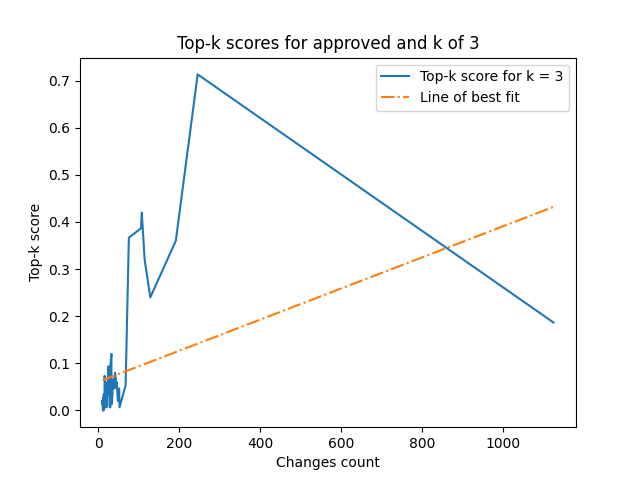
\includegraphics[height=5cm]{images/graphs/rule-based-top-k-approved-k-3.png} }}%
    \subfloat[\centering Without mediawiki/core.]{{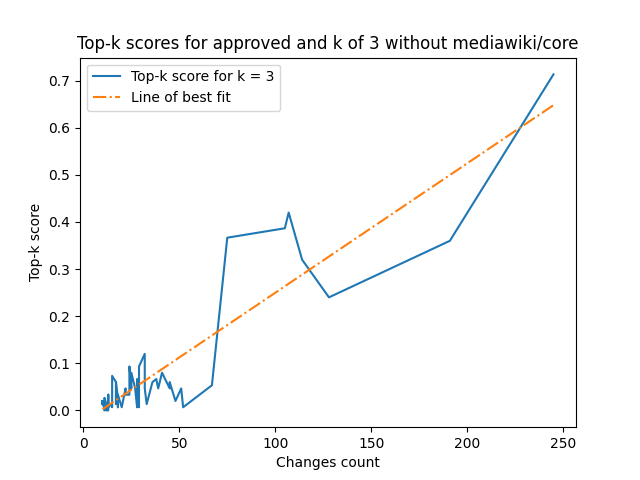
\includegraphics[height=5cm]{images/graphs/rule-based-top-k-approved-k-3-no-core.png} }}%
    \caption{Rule based recommender Top-k score for correctly predicting approvers where k is 3.}%
    \label{fig:rule-based-top-k-approved-k-3-appendix-c}%
\end{figure}

\begin{figure}[H]%
    \centering
    \subfloat[\centering All repositories.]{{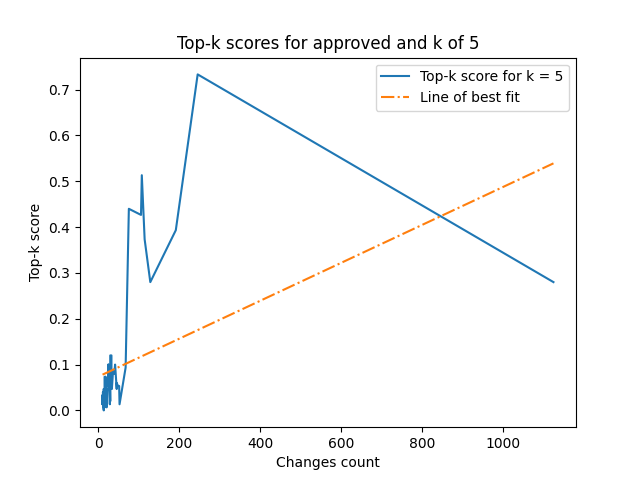
\includegraphics[height=5cm]{images/graphs/rule-based-top-k-approved-k-5.png} }}%
    \subfloat[\centering Without mediawiki/core.]{{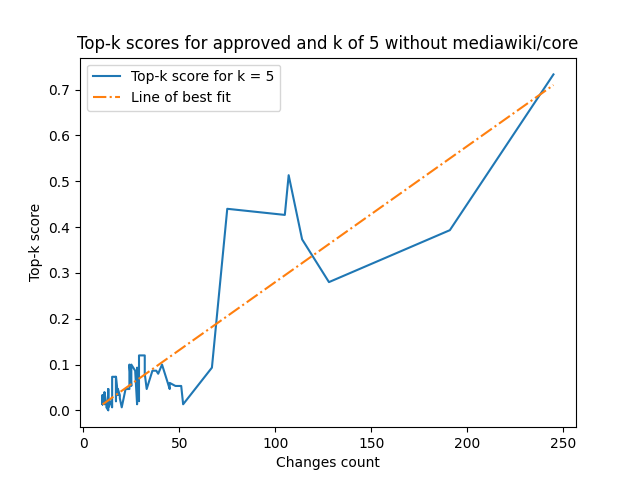
\includegraphics[height=5cm]{images/graphs/rule-based-top-k-approved-k-5-no-core.png} }}%
    \caption{Rule based recommender Top-k score for correctly predicting approvers where k is 5.}%
    \label{fig:rule-based-top-k-approved-k-5-appendix-c}%
\end{figure}

\hspace{0.25cm}
\begin{tabular}{@{}c c c c c@{}} 
 \hline
    \textbf{Repository} &
    \multicolumn{4}{c}{\textbf{Voted}} \\
      & {Top-1} & {Top-3} & {Top-5} & {Top-10} \\
      \hline
mediawiki/extensions/Form & 0.027 & 0.047 & 0.047 & 0.08 \\
mediawiki/extensions/CharRangeSpan & 0.02 & 0.033 & 0.047 & 0.093 \\
mediawiki/extensions/Awesomeness & 0.02 & 0.033 & 0.04 & 0.067 \\
mediawiki/extensions/BlockInactive & 0 & 0 & 0.013 & 0.02 \\
mediawiki/extensions/EtherpadLite & 0 & 0.007 & 0.007 & 0.04 \\
mediawiki/extensions/CheckUser & 0.307 & 0.4 & 0.433 & 0.447 \\
mediawiki/extensions/HashTables & 0 & 0.02 & 0.033 & 0.053 \\
mediawiki/extensions/SemanticACL & 0.027 & 0.047 & 0.053 & 0.08 \\
mediawiki/extensions/LanguageSelector & 0.013 & 0.027 & 0.033 & 0.08 \\
mediawiki/extensions/Disambiguator & 0.087 & 0.293 & 0.333 & 0.387 \\
mediawiki/extensions/SelectTag & 0.007 & 0.02 & 0.033 & 0.107 \\
mediawiki/extensions/I18nTags & 0.027 & 0.067 & 0.1 & 0.153 \\
mediawiki/extensions/CongressLookup & 0.033 & 0.073 & 0.14 & 0.247 \\
mediawiki/extensions/MyVariables & 0.02 & 0.02 & 0.053 & 0.107 \\
mediawiki/extensions/JSBreadCrumbs & 0.02 & 0.06 & 0.06 & 0.1 \\
mediawiki/extensions/SiteSettings & 0.013 & 0.027 & 0.04 & 0.087 \\
mediawiki/extensions/SecureHTML & 0.007 & 0.02 & 0.053 & 0.093 \\
mediawiki/extensions/ShoutWikiAds & 0.02 & 0.02 & 0.02 & 0.02 \\
mediawiki/extensions/BlueSpiceInsertFile & 0 & 0 & 0 & 0.007 \\
mediawiki/extensions/BlueSpiceSocialTimelineUpdate & 0 & 0.007 & 0.007 & 0.02 \\
mediawiki/extensions/WhoIsWatching & 0.007 & 0.013 & 0.013 & 0.027 \\
mediawiki/extensions/ThrottleOverride & 0.02 & 0.027 & 0.04 & 0.047 \\
mediawiki/extensions/UnlinkedWikibase & 0.007 & 0.013 & 0.02 & 0.02 \\
mediawiki/skins/Metrolook & 0.007 & 0.027 & 0.033 & 0.047 \\
mediawiki/extensions/Renameuser & 0.013 & 0.02 & 0.027 & 0.033 \\
mediawiki/extensions/LDAPAuthorization & 0.013 & 0.013 & 0.013 & 0.013 \\
mediawiki/skins/Pivot & 0 & 0.007 & 0.007 & 0.027 \\
mediawiki/extensions/BlueSpiceWikiExplorer & 0 & 0.047 & 0.047 & 0.067 \\
mediawiki/services/texvcjs & 0.053 & 0.38 & 0.44 & 0.473 \\
mediawiki/extensions/Lingo & 0.007 & 0.027 & 0.06 & 0.06 \\
mediawiki/extensions/Wikisource & 0.027 & 0.067 & 0.08 & 0.087 \\
mediawiki/extensions/WebDAV & 0.067 & 0.12 & 0.12 & 0.133 \\
mediawiki/extensions/LegalLogin & 0.02 & 0.033 & 0.047 & 0.073 \\
mediawiki/extensions/BlueSpiceNSFileRepoConnector & 0.007 & 0.02 & 0.027 & 0.033 \\
mediawiki/extensions/MassMessage & 0.033 & 0.087 & 0.107 & 0.14 \\
mediawiki/extensions/LiquidThreads & 0.013 & 0.06 & 0.087 & 0.113 \\
mediawiki/extensions/WikimediaIncubator & 0.013 & 0.047 & 0.053 & 0.093 \\
mediawiki/extensions/cldr & 0.02 & 0.033 & 0.053 & 0.06 \\
\end{tabular}

\begin{tabular}{@{}c c c c c@{}} 
 \hline
    \textbf{Repository} &
    \multicolumn{4}{c}{\textbf{Voted}} \\
      & {Top-1} & {Top-3} & {Top-5} & {Top-10} \\
      \hline
mediawiki/extensions/WikiEditor & 0 & 0.007 & 0.027 & 0.033 \\
mediawiki/extensions/BlueSpicePermissionManager & 0.02 & 0.02 & 0.02 & 0.04 \\
mediawiki/extensions/BlueSpiceInsertCategory & 0.007 & 0.013 & 0.02 & 0.027 \\
mediawiki/skins/TuleapSkin & 0.04 & 0.073 & 0.073 & 0.08 \\
mediawiki/extensions/BlueSpiceSocialTags & 0 & 0.013 & 0.013 & 0.02 \\
mediawiki/extensions/BlueSpiceReaders & 0.013 & 0.02 & 0.02 & 0.027 \\
mediawiki/extensions/BlueSpiceUserManager & 0 & 0.007 & 0.007 & 0.02 \\
mediawiki/extensions/LDAPProvider & 0.04 & 0.06 & 0.073 & 0.073 \\
mediawiki/extensions/BlueSpiceUsageTracker & 0 & 0 & 0.007 & 0.007 \\
mediawiki/extensions/Translate & 0.227 & 0.46 & 0.533 & 0.553 \\
mediawiki/extensions/EnhancedUpload & 0.013 & 0.053 & 0.08 & 0.093 \\
mediawiki/extensions/AbuseFilter & 0.02 & 0.04 & 0.053 & 0.073 \\
mediawiki/extensions/TimedMediaHandler & 0.033 & 0.067 & 0.093 & 0.12 \\
mediawiki/extensions/PageTriage & 0.04 & 0.08 & 0.113 & 0.147 \\
mediawiki/extensions/BlueSpiceRSSFeeder & 0.027 & 0.093 & 0.1 & 0.107 \\
mediawiki/extensions/Wikistories & 0.087 & 0.12 & 0.14 & 0.147 \\
mediawiki/libs/less.php & 0.04 & 0.093 & 0.113 & 0.127 \\
mediawiki/extensions/CentralAuth & 0.033 & 0.047 & 0.087 & 0.1 \\
mediawiki/extensions/Workflows & 0.013 & 0.06 & 0.06 & 0.1 \\
mediawiki/core & 0.08 & 0.2 & 0.3 & 0.44 \\
mediawiki/extensions/GrowthExperiments & 0.44 & 0.74 & 0.76 & 0.767 \\
mediawiki/skins/Vector & 0.167 & 0.38 & 0.413 & 0.547 \\
mediawiki/extensions/VisualEditor & 0.213 & 0.333 & 0.387 & 0.393 \\
\hline
\end{tabular}
\end{center}

Graphs with k equal to 3 and 5 are shown here because they were similar to k equal to 10, and therefore would make more efficient use of space to be here. Figure~\ref{fig:rule-based-top-k-voted-k-1} is the graph for k equal to 1 and Figure~\ref{fig:rule-based-top-k-voted-k-10} is the graph for k equal to 10.

\begin{figure}[H]%
    \centering
    \subfloat[\centering All repositories.]{{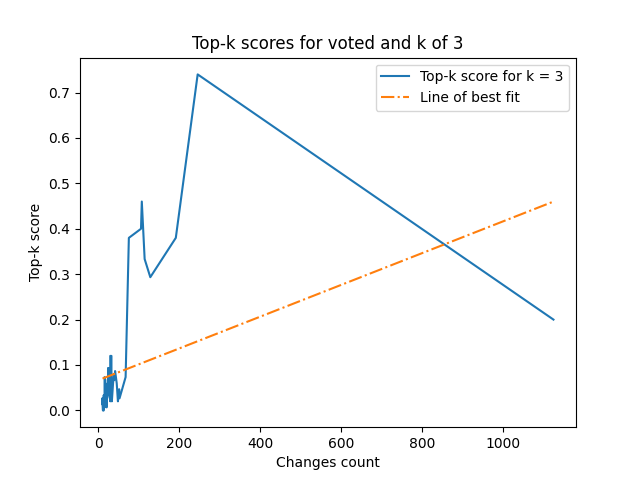
\includegraphics[height=5cm]{images/graphs/rule-based-top-k-voted-k-3.png} }}%
    \subfloat[\centering Without mediawiki/core.]{{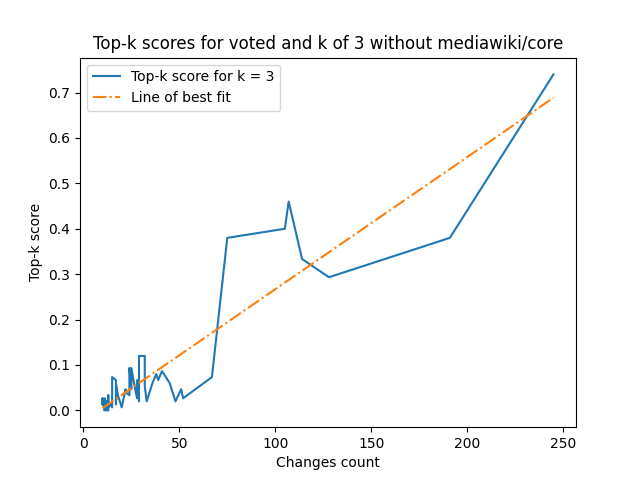
\includegraphics[height=5cm]{images/graphs/rule-based-top-k-voted-k-3-no-core.png} }}%
    \caption{Rule based recommender Top-k score for correctly predicting voters where k is 3.}%
    \label{fig:rule-based-top-k-voted-k-3-appendix-c}%
\end{figure}

\begin{figure}[H]%
    \centering
    \subfloat[\centering All repositories.]{{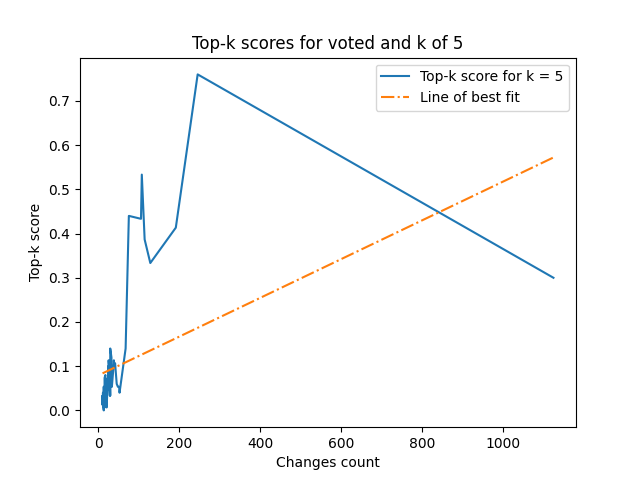
\includegraphics[height=5cm]{images/graphs/rule-based-top-k-voted-k-5.png} }}%
    \subfloat[\centering Without mediawiki/core.]{{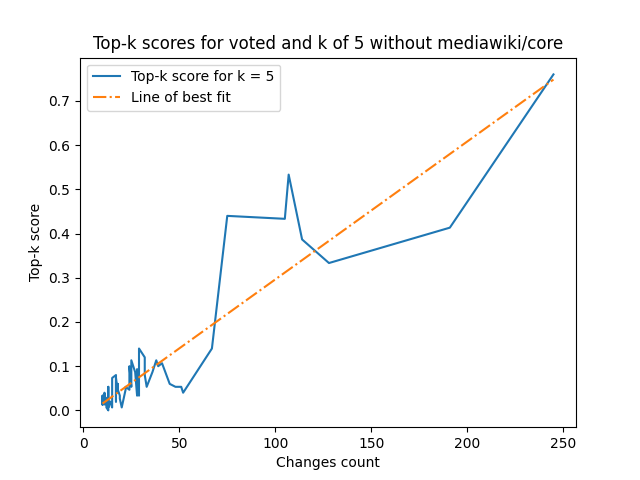
\includegraphics[height=5cm]{images/graphs/rule-based-top-k-voted-k-5-no-core.png} }}%
    \caption{Rule based recommender Top-k score for correctly predicting voters where k is 5.}%
    \label{fig:rule-based-top-k-voted-k-5-appendix-c}%
\end{figure}

\subsubsection{Open changes}
\begin{center}
\hspace{0.25cm}
\begin{tabular}{@{}c c c c c@{}} 
 \hline
    \textbf{Repository} &
    \multicolumn{4}{c}{\textbf{Approved}} \\
      & {Top-1} & {Top-3} & {Top-5} & {Top-10} \\
      \hline
mediawiki/extensions/CheckUser & 0 & 0 & 0 & 0 \\
mediawiki/extensions/Translate & 0 & 0 & 0 & 0 \\
mediawiki/extensions/AbuseFilter & 0 & 0 & 0 & 0 \\
mediawiki/extensions/TimedMediaHandler & 0 & 0 & 0 & 0 \\
mediawiki/extensions/CentralAuth & 0 & 0 & 0 & 0 \\
mediawiki/core & 0 & 0 & 0 & 0.007 \\
mediawiki/extensions/GrowthExperiments & 0.007 & 0.007 & 0.007 & 0.007 \\
mediawiki/skins/Vector & 0 & 0 & 0 & 0 \\
mediawiki/extensions/VisualEditor & 0 & 0 & 0 & 0 \\
\hline
\end{tabular}

\hspace{0.25cm}
\begin{tabular}{@{}c c c c c@{}} 
 \hline
    \textbf{Repository} &
    \multicolumn{4}{c}{\textbf{Voted}} \\
      & {Top-1} & {Top-3} & {Top-5} & {Top-10} \\
      \hline
mediawiki/extensions/CheckUser & 0.007 & 0.013 & 0.013 & 0.013 \\
mediawiki/extensions/Translate & 0.007 & 0.02 & 0.02 & 0.02 \\
mediawiki/extensions/AbuseFilter & 0.007 & 0.013 & 0.013 & 0.013 \\
mediawiki/extensions/TimedMediaHandler & 0.007 & 0.007 & 0.007 & 0.013 \\
mediawiki/extensions/CentralAuth & 0.007 & 0.007 & 0.013 & 0.013 \\
mediawiki/core & 0.133 & 0.273 & 0.307 & 0.393 \\
mediawiki/extensions/GrowthExperiments & 0.02 & 0.027 & 0.027 & 0.027 \\
mediawiki/skins/Vector & 0.013 & 0.02 & 0.027 & 0.027 \\
mediawiki/extensions/VisualEditor & 0.007 & 0.007 & 0.007 & 0.007 \\
\hline
\end{tabular}
\end{center}

\subsubsection{Abandoned changes}
\begin{center}
\hspace{0.25cm}
\begin{tabular}{@{}c c c c c@{}} 
 \hline
    \textbf{Repository} &
    \multicolumn{4}{c}{\textbf{Approved}} \\
      & {Top-1} & {Top-3} & {Top-5} & {Top-10} \\
      \hline
mediawiki/extensions/HashTables & 0 & 0 & 0 & 0 \\
mediawiki/extensions/LanguageSelector & 0 & 0 & 0 & 0 \\
mediawiki/extensions/Disambiguator & 0 & 0 & 0 & 0 \\
mediawiki/extensions/SiteSettings & 0 & 0 & 0 & 0 \\
mediawiki/extensions/MassMessage & 0 & 0 & 0 & 0 \\
mediawiki/extensions/WikimediaIncubator & 0 & 0 & 0 & 0 \\
mediawiki/extensions/AbuseFilter & 0 & 0 & 0.007 & 0.007 \\
mediawiki/extensions/PageTriage & 0 & 0 & 0 & 0 \\
mediawiki/core & 0 & 0.007 & 0.007 & 0.007 \\
mediawiki/extensions/GrowthExperiments & 0 & 0 & 0 & 0.007 \\
mediawiki/skins/Vector & 0 & 0 & 0 & 0 \\
mediawiki/extensions/VisualEditor & 0 & 0 & 0 & 0 \\
\hline
\end{tabular}

\hspace{0.25cm}
\begin{tabular}{@{}c c c c c@{}} 
 \hline
    \textbf{Repository} &
    \multicolumn{4}{c}{\textbf{Voted}} \\
      & {Top-1} & {Top-3} & {Top-5} & {Top-10} \\
      \hline
mediawiki/extensions/HashTables & 0 & 0 & 0 & 0 \\
mediawiki/extensions/LanguageSelector & 0 & 0 & 0 & 0 \\
mediawiki/extensions/Disambiguator & 0 & 0 & 0 & 0 \\
mediawiki/extensions/SiteSettings & 0 & 0 & 0 & 0 \\
mediawiki/extensions/MassMessage & 0.007 & 0.02 & 0.02 & 0.02 \\
mediawiki/extensions/WikimediaIncubator & 0 & 0.02 & 0.02 & 0.02 \\
mediawiki/extensions/AbuseFilter & 0.007 & 0.007 & 0.013 & 0.013 \\
mediawiki/extensions/PageTriage & 0.02 & 0.02 & 0.02 & 0.02 \\
mediawiki/core & 0.107 & 0.153 & 0.16 & 0.193 \\
mediawiki/extensions/GrowthExperiments & 0.04 & 0.047 & 0.047 & 0.047 \\
mediawiki/skins/Vector & 0.033 & 0.04 & 0.04 & 0.04 \\
mediawiki/extensions/VisualEditor & 0.013 & 0.02 & 0.02 & 0.02 \\
\hline
\end{tabular}
\end{center}

\subsection{Neural network recommender}
\begin{center}
\begin{tabular}{@{}c c c c c@{}} 
 \hline
    \textbf{Repository} &
    \multicolumn{4}{c}{\textbf{Approved}} \\
      & {Top-1} & {Top-3} & {Top-5} & {Top-10} \\
      \hline
mediawiki/extensions/Form & 0.05 & 0.1 & 0.11 & 0.13 \\
mediawiki/extensions/CharRangeSpan & 0 & 0.01 & 0.01 & 0.02 \\
mediawiki/extensions/Awesomeness & 0.03 & 0.05 & 0.06 & 0.11 \\
mediawiki/extensions/BlockInactive & 0 & 0 & 0.01 & 0.04 \\
mediawiki/extensions/EtherpadLite & 0.05 & 0.06 & 0.06 & 0.1 \\
mediawiki/extensions/CheckUser & 0.23 & 0.26 & 0.27 & 0.29 \\
mediawiki/extensions/HashTables & 0.01 & 0.06 & 0.08 & 0.08 \\
mediawiki/extensions/SemanticACL & 0 & 0 & 0 & 0.04 \\
mediawiki/extensions/LanguageSelector & 0.05 & 0.06 & 0.08 & 0.12 \\
mediawiki/extensions/Disambiguator & 0.18 & 0.32 & 0.36 & 0.49 \\
mediawiki/extensions/SelectTag & 0 & 0.1 & 0.12 & 0.17 \\
mediawiki/extensions/I18nTags & 0.05 & 0.13 & 0.16 & 0.2 \\
mediawiki/extensions/CongressLookup & 0.01 & 0.02 & 0.04 & 0.04 \\
mediawiki/extensions/MyVariables & 0.06 & 0.12 & 0.17 & 0.22 \\
mediawiki/extensions/JSBreadCrumbs & 0 & 0 & 0.03 & 0.1 \\
mediawiki/extensions/SiteSettings & 0.07 & 0.07 & 0.12 & 0.2 \\
mediawiki/extensions/SecureHTML & 0.01 & 0.07 & 0.09 & 0.12 \\
mediawiki/extensions/ShoutWikiAds & 0.02 & 0.02 & 0.02 & 0.02 \\
mediawiki/extensions/BlueSpiceInsertFile & 0 & 0.01 & 0.01 & 0.01 \\
mediawiki/extensions/BlueSpiceSocialTimelineUpdate & 0.01 & 0.01 & 0.02 & 0.03 \\
mediawiki/extensions/WhoIsWatching & 0.01 & 0.03 & 0.04 & 0.04 \\
mediawiki/extensions/ThrottleOverride & 0.05 & 0.07 & 0.09 & 0.09 \\
mediawiki/extensions/UnlinkedWikibase & 0.01 & 0.03 & 0.03 & 0.03 \\
mediawiki/skins/Metrolook & 0 & 0.02 & 0.03 & 0.05 \\
mediawiki/extensions/Renameuser & 0 & 0.01 & 0.02 & 0.03 \\
mediawiki/extensions/LDAPAuthorization & 0 & 0.01 & 0.01 & 0.01 \\
mediawiki/skins/Pivot & 0 & 0 & 0 & 0 \\
mediawiki/extensions/BlueSpiceWikiExplorer & 0.05 & 0.07 & 0.07 & 0.08 \\
mediawiki/services/texvcjs & 0.51 & 0.63 & 0.68 & 0.68 \\
mediawiki/extensions/Lingo & 0.02 & 0.05 & 0.05 & 0.07 \\
mediawiki/extensions/Wikisource & 0.06 & 0.09 & 0.09 & 0.11 \\
mediawiki/extensions/WebDAV & 0.05 & 0.07 & 0.07 & 0.07 \\
mediawiki/extensions/LegalLogin & 0.02 & 0.07 & 0.09 & 0.12 \\
mediawiki/extensions/BlueSpiceNSFileRepoConnector & 0.01 & 0.04 & 0.05 & 0.05 \\
mediawiki/extensions/MassMessage & 0.17 & 0.25 & 0.27 & 0.31 \\
mediawiki/extensions/LiquidThreads & 0 & 0.06 & 0.13 & 0.2 \\
mediawiki/extensions/WikimediaIncubator & 0.06 & 0.1 & 0.1 & 0.1 \\
\hline
\end{tabular}
\end{center}

\begin{center}
\begin{tabular}{@{}c c c c c@{}} 
 \hline
    \textbf{Repository} &
    \multicolumn{4}{c}{\textbf{Approved}} \\
      & {Top-1} & {Top-3} & {Top-5} & {Top-10} \\
      \hline
mediawiki/extensions/cldr & 0.01 & 0.06 & 0.07 & 0.08 \\
mediawiki/extensions/WikiEditor & 0 & 0.02 & 0.02 & 0.02 \\
mediawiki/extensions/BlueSpicePermissionManager & 0.01 & 0.01 & 0.01 & 0.01 \\
mediawiki/extensions/BlueSpiceInsertCategory & 0.02 & 0.03 & 0.03 & 0.03 \\
mediawiki/skins/TuleapSkin & 0.02 & 0.02 & 0.02 & 0.02 \\
mediawiki/extensions/BlueSpiceSocialTags & 0 & 0 & 0 & 0 \\
mediawiki/extensions/BlueSpiceReaders & 0.02 & 0.02 & 0.02 & 0.02 \\
mediawiki/extensions/BlueSpiceUserManager & 0 & 0 & 0 & 0 \\
mediawiki/extensions/LDAPProvider & 0.01 & 0.01 & 0.01 & 0.01 \\
mediawiki/extensions/BlueSpiceUsageTracker & 0.01 & 0.01 & 0.01 & 0.01 \\
mediawiki/extensions/Translate & 0.6 & 0.74 & 0.75 & 0.77 \\
mediawiki/extensions/EnhancedUpload & 0.06 & 0.06 & 0.07 & 0.07 \\
mediawiki/extensions/AbuseFilter & 0.02 & 0.06 & 0.07 & 0.1 \\
mediawiki/extensions/TimedMediaHandler & 0 & 0 & 0.02 & 0.02 \\
mediawiki/extensions/PageTriage & 0.11 & 0.21 & 0.23 & 0.27 \\
mediawiki/extensions/BlueSpiceRSSFeeder & 0.01 & 0.04 & 0.05 & 0.05 \\
mediawiki/extensions/Wikistories & 0 & 0.08 & 0.11 & 0.11 \\
mediawiki/libs/less.php & 0.02 & 0.02 & 0.02 & 0.02 \\
mediawiki/extensions/CentralAuth & 0.02 & 0.02 & 0.02 & 0.02 \\
mediawiki/extensions/Workflows & 0.03 & 0.06 & 0.06 & 0.06 \\
mediawiki/core & 0.04 & 0.07 & 0.09 & 0.13 \\
mediawiki/extensions/GrowthExperiments & 0.41 & 0.6 & 0.6 & 0.6 \\
mediawiki/skins/Vector & 0 & 0.19 & 0.2 & 0.23 \\
mediawiki/extensions/VisualEditor & 0.28 & 0.35 & 0.4 & 0.45 \\
\hline
\end{tabular}
\end{center}

Graphs with k equal to 3 and 5 are shown here because they were similar to k equal to 10, and therefore would make more efficient use of space to be here. Figure~\ref{fig:neural-network-top-k-approved-k-1} is the graph for k equal to 1 and Figure~\ref{fig:neural-network-top-k-approved-k-10} is the graph for k equal to 10.

\begin{figure}[H]%
    \centering
    \subfloat[\centering All repositories.]{{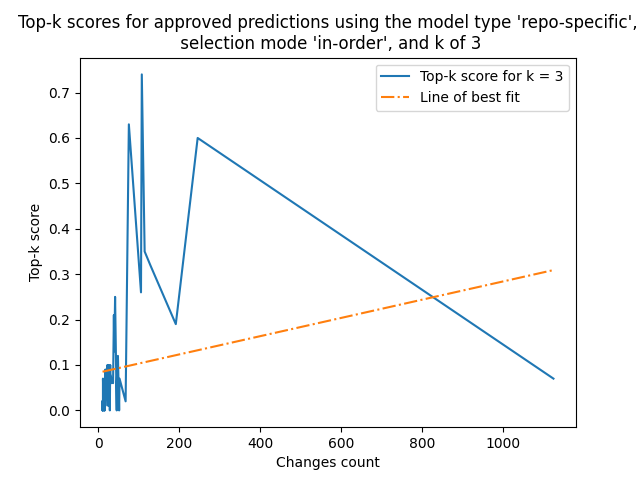
\includegraphics[height=5cm]{images/graphs/neural-network-top-k-approved-k-3-model-mode-repo-specific-selection-mode-in-order.png} }}%
    \subfloat[\centering Without mediawiki/core.]{{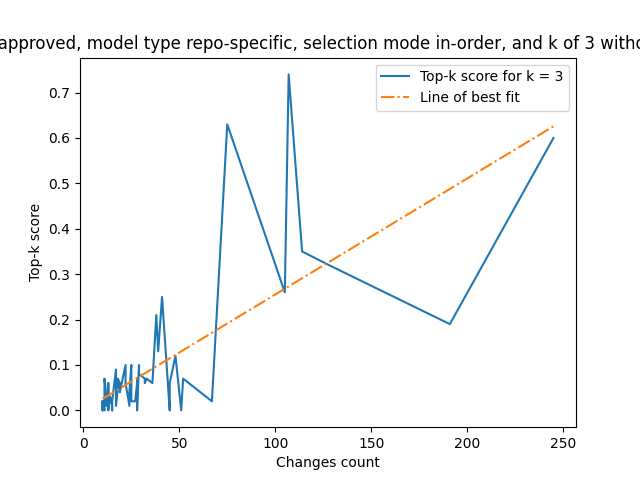
\includegraphics[height=5cm]{images/graphs/neural-network-top-k-approved-k-3-model-mode-repo-specific-selection-mode-in-order-no-core.png} }}%
    \caption{Neural network recommender Top-k score for correctly predicting approvers where k is 3.}%
    \label{fig:neural-network-top-k-approved-k-3-appendix-c}%
\end{figure}

\begin{figure}[H]%
    \centering
    \subfloat[\centering All repositories.]{{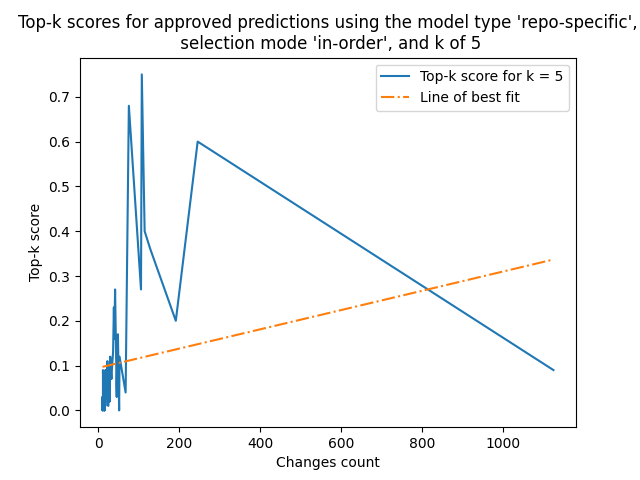
\includegraphics[height=5cm]{images/graphs/neural-network-top-k-approved-k-5-model-mode-repo-specific-selection-mode-in-order.png} }}%
    \subfloat[\centering Without mediawiki/core.]{{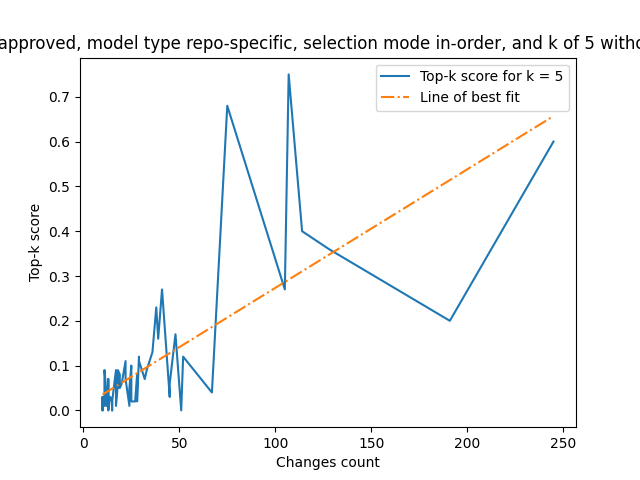
\includegraphics[height=5cm]{images/graphs/neural-network-top-k-approved-k-5-model-mode-repo-specific-selection-mode-in-order-no-core.png} }}%
    \caption{Neural network recommender Top-k score for correctly predicting approvers where k is 5.}%
    \label{fig:neural-network-top-k-approved-k-5-appendix-c}%
\end{figure}

\begin{center}
\begin{tabular}{@{}c c c c c@{}} 
 \hline
    \textbf{Repository} &
    \multicolumn{4}{c}{\textbf{Voted}} \\
      & {Top-1} & {Top-3} & {Top-5} & {Top-10} \\
      \hline
mediawiki/extensions/Form & 0.05 & 0.1 & 0.11 & 0.13 \\
mediawiki/extensions/CharRangeSpan & 0.01 & 0.03 & 0.04 & 0.05 \\
mediawiki/extensions/Awesomeness & 0.03 & 0.05 & 0.07 & 0.11 \\
mediawiki/extensions/BlockInactive & 0 & 0 & 0.01 & 0.04 \\
mediawiki/extensions/EtherpadLite & 0.07 & 0.08 & 0.08 & 0.12 \\
mediawiki/extensions/CheckUser & 0.24 & 0.27 & 0.27 & 0.29 \\
mediawiki/extensions/HashTables & 0.02 & 0.07 & 0.08 & 0.08 \\
mediawiki/extensions/SemanticACL & 0 & 0.01 & 0.02 & 0.06 \\
mediawiki/extensions/LanguageSelector & 0.05 & 0.06 & 0.09 & 0.14 \\
mediawiki/extensions/Disambiguator & 0.22 & 0.4 & 0.44 & 0.62 \\
mediawiki/extensions/SelectTag & 0 & 0.11 & 0.13 & 0.18 \\
mediawiki/extensions/I18nTags & 0.06 & 0.16 & 0.19 & 0.23 \\
mediawiki/extensions/CongressLookup & 0.01 & 0.03 & 0.05 & 0.05 \\
mediawiki/extensions/MyVariables & 0.06 & 0.13 & 0.2 & 0.24 \\
mediawiki/extensions/JSBreadCrumbs & 0 & 0 & 0.05 & 0.12 \\
mediawiki/extensions/SiteSettings & 0.11 & 0.11 & 0.18 & 0.25 \\
mediawiki/extensions/SecureHTML & 0.01 & 0.07 & 0.09 & 0.13 \\
mediawiki/extensions/ShoutWikiAds & 0.02 & 0.02 & 0.02 & 0.02 \\
mediawiki/extensions/BlueSpiceInsertFile & 0 & 0.01 & 0.01 & 0.01 \\
mediawiki/extensions/BlueSpiceSocialTimelineUpdate & 0.01 & 0.01 & 0.02 & 0.03 \\
mediawiki/extensions/WhoIsWatching & 0.01 & 0.03 & 0.04 & 0.04 \\
mediawiki/extensions/ThrottleOverride & 0.05 & 0.07 & 0.09 & 0.09 \\
mediawiki/extensions/UnlinkedWikibase & 0.01 & 0.03 & 0.03 & 0.03 \\
mediawiki/skins/Metrolook & 0 & 0.02 & 0.04 & 0.05 \\
mediawiki/extensions/Renameuser & 0 & 0.03 & 0.04 & 0.05 \\
mediawiki/extensions/LDAPAuthorization & 0 & 0.01 & 0.01 & 0.01 \\
mediawiki/skins/Pivot & 0 & 0 & 0 & 0 \\
mediawiki/extensions/BlueSpiceWikiExplorer & 0.05 & 0.07 & 0.07 & 0.08 \\
mediawiki/services/texvcjs & 0.53 & 0.63 & 0.68 & 0.68 \\
mediawiki/extensions/Lingo & 0.04 & 0.07 & 0.07 & 0.09 \\
mediawiki/extensions/Wikisource & 0.06 & 0.1 & 0.1 & 0.12 \\
mediawiki/extensions/WebDAV & 0.05 & 0.07 & 0.07 & 0.07 \\
mediawiki/extensions/LegalLogin & 0.02 & 0.07 & 0.09 & 0.12 \\
mediawiki/extensions/BlueSpiceNSFileRepoConnector & 0.01 & 0.04 & 0.05 & 0.05 \\
mediawiki/extensions/MassMessage & 0.17 & 0.25 & 0.28 & 0.31 \\
\hline
\end{tabular}
\end{center}

\begin{center}
\begin{tabular}{@{}c c c c c@{}} 
 \hline
    \textbf{Repository} &
    \multicolumn{4}{c}{\textbf{Voted}} \\
      & {Top-1} & {Top-3} & {Top-5} & {Top-10} \\
      \hline
mediawiki/extensions/LiquidThreads & 0 & 0.06 & 0.13 & 0.21 \\
mediawiki/extensions/WikimediaIncubator & 0.06 & 0.1 & 0.1 & 0.1 \\
mediawiki/extensions/cldr & 0.02 & 0.07 & 0.07 & 0.08 \\
mediawiki/extensions/WikiEditor & 0 & 0.02 & 0.02 & 0.02 \\
mediawiki/extensions/BlueSpicePermissionManager & 0.01 & 0.01 & 0.01 & 0.01 \\
mediawiki/extensions/BlueSpiceInsertCategory & 0.02 & 0.03 & 0.03 & 0.03 \\
mediawiki/skins/TuleapSkin & 0.02 & 0.02 & 0.02 & 0.02 \\
mediawiki/extensions/BlueSpiceSocialTags & 0 & 0 & 0 & 0 \\
mediawiki/extensions/BlueSpiceReaders & 0.02 & 0.02 & 0.02 & 0.02 \\
mediawiki/extensions/BlueSpiceUserManager & 0 & 0 & 0 & 0 \\
mediawiki/extensions/LDAPProvider & 0.01 & 0.01 & 0.01 & 0.01 \\
mediawiki/extensions/BlueSpiceUsageTracker & 0.01 & 0.01 & 0.01 & 0.01 \\
mediawiki/extensions/Translate & 0.63 & 0.77 & 0.78 & 0.79 \\
mediawiki/extensions/EnhancedUpload & 0.07 & 0.07 & 0.07 & 0.07 \\
mediawiki/extensions/AbuseFilter & 0.02 & 0.06 & 0.08 & 0.1 \\
mediawiki/extensions/TimedMediaHandler & 0 & 0 & 0.02 & 0.02 \\
mediawiki/extensions/PageTriage & 0.11 & 0.21 & 0.24 & 0.28 \\
mediawiki/extensions/BlueSpiceRSSFeeder & 0.01 & 0.04 & 0.05 & 0.05 \\
mediawiki/extensions/Wikistories & 0 & 0.13 & 0.16 & 0.16 \\
mediawiki/libs/less.php & 0.02 & 0.02 & 0.02 & 0.02 \\
mediawiki/extensions/CentralAuth & 0.02 & 0.03 & 0.03 & 0.03 \\
mediawiki/extensions/Workflows & 0.03 & 0.06 & 0.06 & 0.06 \\
mediawiki/core & 0.05 & 0.08 & 0.1 & 0.16 \\
mediawiki/extensions/GrowthExperiments & 0.44 & 0.62 & 0.62 & 0.63 \\
mediawiki/skins/Vector & 0 & 0.21 & 0.22 & 0.25 \\
mediawiki/extensions/VisualEditor & 0.3 & 0.39 & 0.44 & 0.49 \\
\hline
\end{tabular}
\end{center}

Graphs with k equal to 3 and 5 are shown here because they were similar to k equal to 10, and therefore would make more efficient use of space to be here. Figure~\ref{fig:neural-network-top-k-voted-k-1} is the graph for k equal to 1 and Figure~\ref{fig:neural-network-top-k-voted-k-10} is the graph for k equal to 10.

\begin{figure}[H]%
    \centering
    \subfloat[\centering All repositories.]{{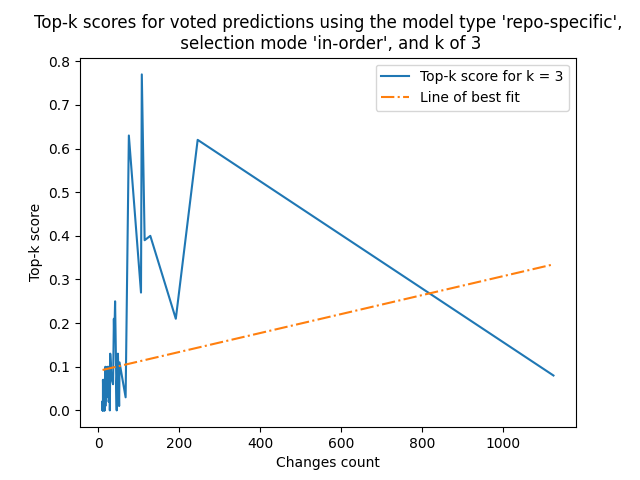
\includegraphics[height=5cm]{images/graphs/neural-network-top-k-voted-k-3-model-mode-repo-specific-selection-mode-in-order.png} }}%
    \subfloat[\centering Without mediawiki/core.]{{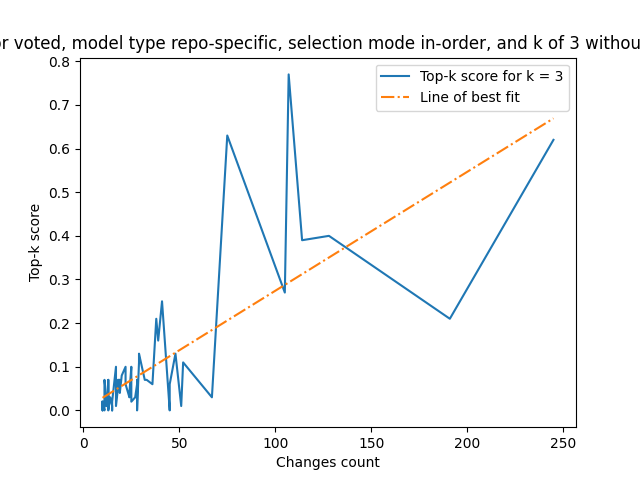
\includegraphics[height=5cm]{images/graphs/neural-network-top-k-voted-k-3-model-mode-repo-specific-selection-mode-in-order-no-core.png} }}%
    \caption{Neural network recommender Top-k score for correctly predicting voters where k is 3.}%
    \label{fig:neural-network-top-k-voted-k-3-appendix-c}%
\end{figure}

\begin{figure}[H]%
    \centering
    \subfloat[\centering All repositories.]{{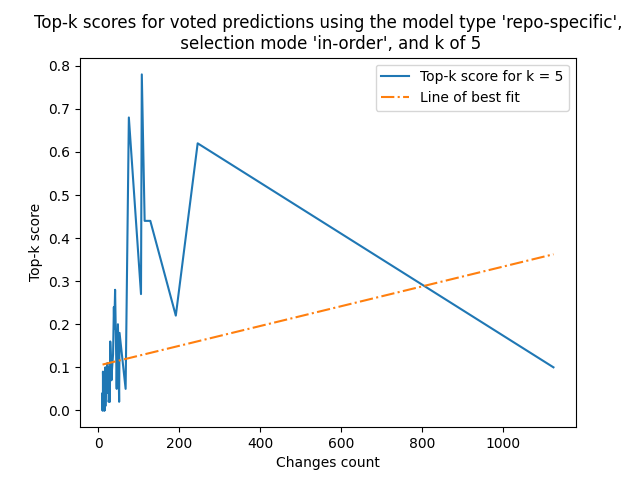
\includegraphics[height=5cm]{images/graphs/neural-network-top-k-voted-k-5-model-mode-repo-specific-selection-mode-in-order.png} }}%
    \subfloat[\centering Without mediawiki/core.]{{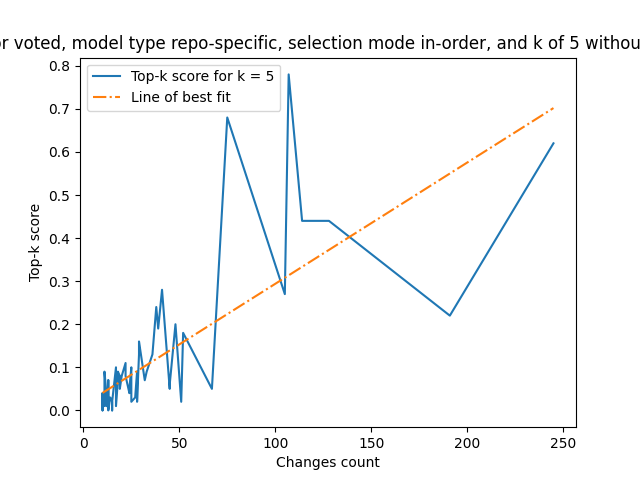
\includegraphics[height=5cm]{images/graphs/neural-network-top-k-voted-k-5-model-mode-repo-specific-selection-mode-in-order-no-core.png} }}%
    \caption{Neural network recommender Top-k score for correctly predicting voters where k is 5.}%
    \label{fig:neural-network-top-k-voted-k-5-appendix-c}%
\end{figure}

\section{MRR score}
\subsection{Rule based recommender}
\subsubsection{Merged changes}
\hspace{0.25cm}
\begin{center}
\begin{tabular}{@{}c c c@{}} 
 \hline
    \textbf{Repository} & {Approved MRR} & {Voted MRR} \\
\hline
mediawiki/extensions/Form & 0.038 & 0.039 \\
mediawiki/extensions/CharRangeSpan & 0.027 & 0.037 \\
mediawiki/extensions/Awesomeness & 0.036 & 0.043 \\
mediawiki/extensions/BlockInactive & 0.004 & 0.004 \\
mediawiki/extensions/EtherpadLite & 0.013 & 0.021 \\
mediawiki/extensions/CheckUser & 0.331 & 0.325 \\
mediawiki/extensions/HashTables & 0.018 & 0.018 \\
mediawiki/extensions/SemanticACL & 0.025 & 0.03 \\
mediawiki/extensions/LanguageSelector & 0.012 & 0.033 \\
mediawiki/extensions/Disambiguator & 0.101 & 0.141 \\
mediawiki/extensions/SelectTag & 0.016 & 0.029 \\
mediawiki/extensions/I18nTags & 0.03 & 0.044 \\
mediawiki/extensions/CongressLookup & 0.036 & 0.063 \\
mediawiki/extensions/MyVariables & 0.041 & 0.051 \\
mediawiki/extensions/JSBreadCrumbs & 0.032 & 0.045 \\
mediawiki/extensions/SiteSettings & 0.042 & 0.073 \\
mediawiki/extensions/SecureHTML & 0.025 & 0.034 \\
mediawiki/extensions/ShoutWikiAds & 0.029 & 0.029 \\
mediawiki/extensions/BlueSpiceInsertFile & 0.001 & 0.001 \\
mediawiki/extensions/BlueSpiceSocialTimelineUpdate & 0.004 & 0.004 \\
mediawiki/extensions/WhoIsWatching & 0.001 & 0.001 \\
mediawiki/extensions/ThrottleOverride & 0.005 & 0.005 \\
mediawiki/extensions/UnlinkedWikibase & 0.004 & 0.004 \\
mediawiki/skins/Metrolook & 0.017 & 0.017 \\
mediawiki/extensions/Renameuser & 0.006 & 0.006 \\
mediawiki/extensions/LDAPAuthorization & 0.007 & 0.007 \\
mediawiki/skins/Pivot & 0.003 & 0.003 \\
mediawiki/extensions/BlueSpiceWikiExplorer & 0.02 & 0.021 \\
mediawiki/services/texvcjs & 0.153 & 0.153 \\
mediawiki/extensions/Lingo & 0.009 & 0.01 \\
mediawiki/extensions/Wikisource & 0.038 & 0.039 \\
mediawiki/extensions/WebDAV & 0.047 & 0.047 \\
mediawiki/extensions/LegalLogin & 0.024 & 0.024 \\
mediawiki/extensions/BlueSpiceNSFileRepoConnector & 0.009 & 0.009 \\
\end{tabular}
\begin{tabular}{@{}c c c@{}} 
 \hline
    \textbf{Repository} & {Approved MRR} & {Voted MRR} \\
\hline
mediawiki/extensions/MassMessage & 0.043 & 0.039 \\
mediawiki/extensions/LiquidThreads & 0.036 & 0.036 \\
mediawiki/extensions/WikimediaIncubator & 0.045 & 0.046 \\
mediawiki/extensions/cldr & 0.026 & 0.026 \\
mediawiki/extensions/WikiEditor & 0.028 & 0.011 \\
mediawiki/extensions/BlueSpicePermissionManager & 0.02 & 0.02 \\
mediawiki/extensions/BlueSpiceInsertCategory & 0.017 & 0.017 \\
mediawiki/skins/TuleapSkin & 0.042 & 0.045 \\
mediawiki/extensions/BlueSpiceSocialTags & 0.004 & 0.004 \\
mediawiki/extensions/BlueSpiceReaders & 0.016 & 0.016 \\
mediawiki/extensions/BlueSpiceUserManager & 0.002 & 0.002 \\
mediawiki/extensions/LDAPProvider & 0.033 & 0.033 \\
mediawiki/extensions/BlueSpiceUsageTracker & 0.004 & 0.004 \\
mediawiki/extensions/Translate & 0.335 & 0.352 \\
mediawiki/extensions/EnhancedUpload & 0.028 & 0.028 \\
mediawiki/extensions/AbuseFilter & 0.018 & 0.02 \\
mediawiki/extensions/TimedMediaHandler & 0.039 & 0.039 \\
mediawiki/extensions/PageTriage & 0.04 & 0.05 \\
mediawiki/extensions/BlueSpiceRSSFeeder & 0.032 & 0.032 \\
mediawiki/extensions/Wikistories & 0.118 & 0.131 \\
mediawiki/libs/less.php & 0.033 & 0.035 \\
mediawiki/extensions/CentralAuth & 0.066 & 0.066 \\
mediawiki/extensions/Workflows & 0.034 & 0.034 \\
mediawiki/core & 0.219 & 0.201 \\
mediawiki/extensions/GrowthExperiments & 0.498 & 0.536 \\
mediawiki/skins/Vector & 0.355 & 0.379 \\
mediawiki/extensions/VisualEditor & 0.229 & 0.247 \\
\hline
\end{tabular}
\end{center}

\subsubsection{Open changes}
\hspace{0.25cm}
\begin{center}
\begin{tabular}{@{}c c c@{}} 
 \hline
    \textbf{Repository} & {Approved MRR} & {Voted MRR} \\
\hline
mediawiki/extensions/CheckUser & 0.0 & 0.007 \\
mediawiki/extensions/Translate & 0.0 & 0.01 \\
mediawiki/extensions/AbuseFilter & 0.0 & 0.008 \\
mediawiki/extensions/TimedMediaHandler & 0.0 & 0.009 \\
mediawiki/extensions/CentralAuth & 0.0 & 0.004 \\
mediawiki/core & 0.002 & 0.193 \\
mediawiki/extensions/GrowthExperiments & 0.001 & 0.018 \\
mediawiki/skins/Vector & 0.0 & 0.017 \\
mediawiki/extensions/VisualEditor & 0.0 & 0.02 \\
 \hline
\end{tabular}
\end{center}

\subsubsection{Abandoned changes}
\hspace{0.25cm}
\begin{center}
\begin{tabular}{@{}c c c@{}} 
 \hline
    \textbf{Repository} & {Approved MRR} & {Voted MRR} \\
\hline
mediawiki/extensions/HashTables & 0.0 & 0.0 \\
mediawiki/extensions/LanguageSelector & 0.0 & 0.0 \\
mediawiki/extensions/Disambiguator & 0.0 & 0.0 \\
mediawiki/extensions/SiteSettings & 0.0 & 0.0 \\
mediawiki/extensions/MassMessage & 0.0 & 0.009 \\
mediawiki/extensions/WikimediaIncubator & 0.0 & 0.02 \\
mediawiki/extensions/AbuseFilter & 0.0 & 0.007 \\
mediawiki/extensions/PageTriage & 0.0 & 0.017 \\
mediawiki/core & 0.007 & 0.115 \\
mediawiki/extensions/GrowthExperiments & 0.002 & 0.033 \\
mediawiki/skins/Vector & 0.007 & 0.022 \\
mediawiki/extensions/VisualEditor & 0.0 & 0.016 \\
 \hline
\end{tabular}
\end{center}

\subsection{Neural network recommender}

\begin{center}
\begin{tabular}{@{}c c c@{}} 
 \hline
    \textbf{Repository} & {Approved MRR} & {Voted MRR} \\
\hline
mediawiki/extensions/Form & 0.083 & 0.083 \\
mediawiki/extensions/CharRangeSpan & 0.038 & 0.065 \\
mediawiki/extensions/Awesomeness & 0.054 & 0.054 \\
mediawiki/extensions/BlockInactive & 0.011 & 0.011 \\
mediawiki/extensions/EtherpadLite & 0.069 & 0.086 \\
mediawiki/extensions/CheckUser & 0.255 & 0.263 \\
mediawiki/extensions/HashTables & 0.054 & 0.06 \\
mediawiki/extensions/SemanticACL & 0.102 & 0.116 \\
mediawiki/extensions/LanguageSelector & 0.072 & 0.073 \\
mediawiki/extensions/Disambiguator & 0.306 & 0.368 \\
mediawiki/extensions/SelectTag & 0.054 & 0.059 \\
mediawiki/extensions/I18nTags & 0.109 & 0.124 \\
mediawiki/extensions/MyVariables & 0.115 & 0.121 \\
mediawiki/extensions/JSBreadCrumbs & 0.046 & 0.064 \\
mediawiki/extensions/SiteSettings & 0.113 & 0.153 \\
mediawiki/extensions/SecureHTML & 0.059 & 0.059 \\
mediawiki/extensions/ShoutWikiAds & 0.021 & 0.021 \\
mediawiki/extensions/BlueSpiceInsertFile & 0.021 & 0.021 \\
mediawiki/extensions/BlueSpiceSocialTimelineUpdate & 0.029 & 0.029 \\
mediawiki/extensions/WhoIsWatching & 0.032 & 0.032 \\
mediawiki/extensions/ThrottleOverride & 0.064 & 0.064 \\
mediawiki/extensions/UnlinkedWikibase & 0.042 & 0.042 \\
mediawiki/skins/Metrolook & 0.012 & 0.012 \\
mediawiki/extensions/Renameuser & 0.018 & 0.026 \\
mediawiki/extensions/LDAPAuthorization & 0.022 & 0.022 \\
mediawiki/skins/Pivot & 0.001 & 0.001 \\
mediawiki/extensions/BlueSpiceWikiExplorer & 0.061 & 0.061 \\
mediawiki/services/texvcjs & 0.584 & 0.594 \\
mediawiki/extensions/Lingo & 0.04 & 0.059 \\
mediawiki/extensions/Wikisource & 0.079 & 0.082 \\
mediawiki/extensions/WebDAV & 0.114 & 0.114 \\
mediawiki/extensions/LegalLogin & 0.055 & 0.055 \\
mediawiki/extensions/BlueSpiceNSFileRepoConnector & 0.028 & 0.028 \\
mediawiki/extensions/MassMessage & 0.224 & 0.226 \\
mediawiki/extensions/LiquidThreads & 0.065 & 0.066 \\
mediawiki/extensions/WikimediaIncubator & 0.076 & 0.076 \\
mediawiki/extensions/cldr & 0.048 & 0.056 \\
 \hline
\end{tabular}
\end{center}

\begin{center}
\begin{tabular}{@{}c c c@{}} 
 \hline
    \textbf{Repository} & {Approved MRR} & {Voted MRR} \\
\hline
mediawiki/extensions/WikiEditor & 0.011 & 0.011 \\
mediawiki/extensions/BlueSpicePermissionManager & 0.033 & 0.033 \\
mediawiki/extensions/BlueSpiceInsertCategory & 0.1 & 0.1 \\
mediawiki/skins/TuleapSkin & 0.021 & 0.021 \\
mediawiki/extensions/BlueSpiceSocialTags & 0.001 & 0.001 \\
mediawiki/extensions/BlueSpiceReaders & 0.095 & 0.095 \\
mediawiki/extensions/BlueSpiceUserManager & 0.001 & 0.001 \\
mediawiki/extensions/Translate & 0.707 & 0.751 \\
mediawiki/extensions/EnhancedUpload & 0.115 & 0.123 \\
mediawiki/extensions/AbuseFilter & 0.045 & 0.046 \\
mediawiki/extensions/TimedMediaHandler & 0.003 & 0.003 \\
mediawiki/extensions/PageTriage & 0.169 & 0.174 \\
mediawiki/extensions/BlueSpiceRSSFeeder & 0.021 & 0.021 \\
mediawiki/extensions/Wikistories & 0.037 & 0.055 \\
mediawiki/libs/less.php & 0.022 & 0.022 \\
mediawiki/extensions/CentralAuth & 0.022 & 0.026 \\
mediawiki/core & 0.073 & 0.078 \\
mediawiki/extensions/GrowthExperiments & 0.502 & 0.532 \\
mediawiki/skins/Vector & 0.119 & 0.135 \\
mediawiki/extensions/VisualEditor & 0.477 & 0.499 \\
 \hline
\end{tabular}
\end{center}

\section{Accuracy score}
\subsection{Predicting approved}
\subsubsection{Repo-specific and generic}
\begin{table}[H]
    \centering
    \begin{tabular}{@{}c c c c@{}} 
    \hline
    \textbf{Repository} & \textbf{Average} & \textbf{Minimum} & \textbf{Maximum} \\
    \hline
Generic & 0.993 & 0.975 & 1.0 \\
mediawiki/extensions/AbuseFilter & 0.143 & 0.066 & 0.29 \\
mediawiki/extensions/Awesomeness & 0.992 & 0.987 & 1.0 \\
mediawiki/extensions/BlockInactive & 0.974 & 0.974 & 0.974 \\
mediawiki/extensions/BlueSpiceInsertCategory & 0.99 & 0.987 & 1.0 \\
mediawiki/extensions/BlueSpiceInsertFile & 0.972 & 0.963 & 0.981 \\
mediawiki/extensions/BlueSpiceNSFileRepoConnector & 0.952 & 0.942 & 0.961 \\
mediawiki/extensions/BlueSpicePermissionManager & 0.989 & 0.987 & 0.994 \\
mediawiki/extensions/BlueSpiceRSSFeeder & 0.955 & 0.942 & 0.967 \\
mediawiki/extensions/BlueSpiceReaders & 0.99 & 0.981 & 0.994 \\
mediawiki/extensions/BlueSpiceSocialTags & 0.044 & 0.044 & 0.045 \\
mediawiki/extensions/BlueSpiceSocialTimelineUpdate & 0.986 & 0.981 & 1.0 \\
mediawiki/extensions/BlueSpiceUsageTracker & 0.983 & 0.975 & 0.994 \\
mediawiki/extensions/BlueSpiceUserManager & 0.062 & 0.038 & 0.08 \\
mediawiki/extensions/BlueSpiceWikiExplorer & 0.985 & 0.973 & 0.987 \\
mediawiki/extensions/CentralAuth & 0.188 & 0.086 & 0.258 \\
mediawiki/extensions/CharRangeSpan & 0.896 & 0.887 & 0.906 \\
mediawiki/extensions/CheckUser & 0.99 & 0.981 & 0.995 \\
mediawiki/extensions/CongressLookup & 0.131 & 0.117 & 0.169 \\
mediawiki/extensions/Disambiguator & 0.19 & 0.172 & 0.215 \\
mediawiki/extensions/EnhancedUpload & 0.988 & 0.981 & 0.994 \\
mediawiki/extensions/EtherpadLite & 0.078 & 0.071 & 0.09 \\
mediawiki/extensions/Form & 0.942 & 0.928 & 0.954 \\
mediawiki/extensions/GrowthExperiments & 0.116 & 0.071 & 0.179 \\
mediawiki/extensions/HashTables & 0.084 & 0.071 & 0.096 \\
mediawiki/extensions/I18nTags & 0.981 & 0.967 & 0.994 \\
mediawiki/extensions/JSBreadCrumbs & 0.893 & 0.877 & 0.906 \\
mediawiki/extensions/LDAPAuthorization & 0.991 & 0.987 & 1.0 \\
mediawiki/extensions/LDAPProvider & 0.988 & 0.981 & 0.994 \\
mediawiki/extensions/LanguageSelector & 0.124 & 0.102 & 0.152 \\
mediawiki/extensions/LegalLogin & 0.983 & 0.974 & 0.987 \\
mediawiki/extensions/Lingo & 0.988 & 0.987 & 0.993 \\
mediawiki/extensions/LiquidThreads & 0.148 & 0.054 & 0.306 \\
mediawiki/extensions/MassMessage & 0.985 & 0.976 & 0.994 \\
mediawiki/extensions/MyVariables & 0.992 & 0.988 & 1.0 \\
mediawiki/extensions/PageTriage & 0.981 & 0.967 & 0.994 \\
mediawiki/extensions/Renameuser & 0.967 & 0.947 & 0.978 \\
\hline
\end{tabular}
    \label{table:accuracy-score-repo-specific-and-generic-appendix-c-part-1}
\end{table}

\begin{table}[H]
    \centering
    \begin{tabular}{@{}c c c c@{}} 
    \hline
    \textbf{Repository} & \textbf{Average} & \textbf{Minimum} & \textbf{Maximum} \\
    \hline
mediawiki/extensions/SecureHTML & 0.99 & 0.98 & 1.0 \\
mediawiki/extensions/SelectTag & 0.977 & 0.967 & 0.987 \\
mediawiki/extensions/SemanticACL & 0.906 & 0.899 & 0.917 \\
mediawiki/extensions/ShoutWikiAds & 0.958 & 0.947 & 0.979 \\
mediawiki/extensions/SiteSettings & 0.987 & 0.969 & 1.0 \\
mediawiki/extensions/ThrottleOverride & 0.976 & 0.955 & 0.993 \\
mediawiki/extensions/TimedMediaHandler & 0.082 & 0.04 & 0.113 \\
mediawiki/extensions/Translate & 0.989 & 0.975 & 1.0 \\
mediawiki/extensions/UnlinkedWikibase & 0.995 & 0.979 & 1.0 \\
mediawiki/extensions/VisualEditor & 0.992 & 0.982 & 1.0 \\
mediawiki/extensions/WebDAV & 0.985 & 0.975 & 0.994 \\
mediawiki/extensions/WhoIsWatching & 0.991 & 0.986 & 1.0 \\
mediawiki/extensions/WikiEditor & 0.115 & 0.06 & 0.149 \\
mediawiki/extensions/WikimediaIncubator & 0.941 & 0.924 & 0.965 \\
mediawiki/extensions/Wikisource & 0.987 & 0.98 & 1.0 \\
mediawiki/extensions/Wikistories & 0.958 & 0.934 & 0.966 \\
mediawiki/extensions/Workflows & 0.992 & 0.981 & 1.0 \\
mediawiki/extensions/cldr & 0.971 & 0.969 & 0.974 \\
mediawiki/core & 0.461 & 0.381 & 0.687 \\
mediawiki/libs/less.php & 0.079 & 0.021 & 0.167 \\
mediawiki/services/texvcjs & 0.989 & 0.967 & 0.994 \\
mediawiki/skins/Metrolook & 0.963 & 0.947 & 0.973 \\
mediawiki/skins/Pivot & 0.068 & 0.046 & 0.083 \\
mediawiki/skins/TuleapSkin & 0.028 & 0.013 & 0.05 \\
mediawiki/skins/Vector & 0.144 & 0.101 & 0.219 \\
    \hline
\end{tabular}
    \label{table:accuracy-score-repo-specific-and-generic-appendix-c-part-2}
\end{table}

\begin{table}[H]
    \centering
    \begin{tabular}{@{}c c c@{}} 
    \hline
    \textbf{Repository} & \textbf{10th percentile} & \textbf{90th percentile} \\
    \hline
    Generic & 0.987 & 0.997 \\
mediawiki/extensions/AbuseFilter & 0.066 & 0.195 \\
mediawiki/extensions/Awesomeness & 0.987 & 1.0 \\
mediawiki/extensions/BlockInactive & 0.974 & 0.974 \\
mediawiki/extensions/BlueSpiceInsertCategory & 0.987 & 1.0 \\
mediawiki/extensions/BlueSpiceInsertFile & 0.963 & 0.981 \\
mediawiki/extensions/BlueSpiceNSFileRepoConnector & 0.942 & 0.961 \\
mediawiki/extensions/BlueSpicePermissionManager & 0.987 & 0.994 \\
mediawiki/extensions/BlueSpiceRSSFeeder & 0.942 & 0.961 \\
mediawiki/extensions/BlueSpiceReaders & 0.981 & 0.994 \\
mediawiki/extensions/BlueSpiceSocialTags & 0.044 & 0.045 \\
    \hline
\end{tabular}
    
    \label{table:accuracy-score-repo-specific-and-generic-appendix-c-part-3}
\end{table}

\begin{table}[H]
    \centering
    \begin{tabular}{@{}c c c@{}} 
    \hline
    \textbf{Repository} & \textbf{10th percentile} & \textbf{90th percentile} \\
    \hline
mediawiki/extensions/BlueSpiceSocialTimelineUpdate & 0.981 & 1.0 \\
mediawiki/extensions/BlueSpiceUsageTracker & 0.975 & 0.994 \\
mediawiki/extensions/BlueSpiceUserManager & 0.038 & 0.08 \\
mediawiki/extensions/BlueSpiceWikiExplorer & 0.973 & 0.987 \\
mediawiki/extensions/CentralAuth & 0.086 & 0.232 \\
mediawiki/extensions/CharRangeSpan & 0.887 & 0.899 \\
mediawiki/extensions/CheckUser & 0.987 & 0.994 \\
mediawiki/extensions/CongressLookup & 0.117 & 0.143 \\
mediawiki/extensions/Disambiguator & 0.179 & 0.203 \\
mediawiki/extensions/EnhancedUpload & 0.981 & 0.994 \\
mediawiki/extensions/EtherpadLite & 0.071 & 0.09 \\
mediawiki/extensions/Form & 0.928 & 0.947 \\
mediawiki/extensions/GrowthExperiments & 0.083 & 0.161 \\
mediawiki/extensions/HashTables & 0.071 & 0.084 \\
mediawiki/extensions/I18nTags & 0.967 & 0.993 \\
mediawiki/extensions/JSBreadCrumbs & 0.877 & 0.9 \\
mediawiki/extensions/LDAPAuthorization & 0.987 & 1.0 \\
mediawiki/extensions/LDAPProvider & 0.981 & 0.994 \\
mediawiki/extensions/LanguageSelector & 0.102 & 0.141 \\
mediawiki/extensions/LegalLogin & 0.974 & 0.987 \\
mediawiki/extensions/Lingo & 0.987 & 0.993 \\
mediawiki/extensions/LiquidThreads & 0.054 & 0.245 \\
mediawiki/extensions/MassMessage & 0.976 & 0.994 \\
mediawiki/extensions/MyVariables & 0.988 & 1.0 \\
mediawiki/extensions/PageTriage & 0.967 & 0.994 \\
mediawiki/extensions/Renameuser & 0.947 & 0.978 \\
mediawiki/extensions/SecureHTML & 0.98 & 1.0 \\
mediawiki/extensions/SelectTag & 0.967 & 0.98 \\
mediawiki/extensions/SemanticACL & 0.899 & 0.917 \\
mediawiki/extensions/ShoutWikiAds & 0.947 & 0.979 \\
mediawiki/extensions/SiteSettings & 0.969 & 1.0 \\
mediawiki/extensions/ThrottleOverride & 0.955 & 0.993 \\
mediawiki/extensions/TimedMediaHandler & 0.04 & 0.107 \\
mediawiki/extensions/Translate & 0.976 & 0.995 \\
mediawiki/extensions/UnlinkedWikibase & 0.979 & 1.0 \\
mediawiki/extensions/VisualEditor & 0.988 & 0.995 \\
mediawiki/extensions/WebDAV & 0.975 & 0.987 \\
mediawiki/extensions/WhoIsWatching & 0.986 & 1.0 \\
mediawiki/extensions/WikiEditor & 0.06 & 0.149 \\
mediawiki/extensions/WikimediaIncubator & 0.924 & 0.955 \\
    \hline
\end{tabular}
    \label{table:accuracy-score-repo-specific-and-generic-appendix-c-part-4}
\end{table}

\begin{table}[H]
    \centering
    \begin{tabular}{@{}c c c c@{}} 
    \hline
    \textbf{Repository} & \textbf{10th percentile} & \textbf{90th percentile} \\
    \hline
    Generic & 0.987 & 0.997 \\
mediawiki/extensions/Wikisource & 0.98 & 1.0 \\
mediawiki/extensions/Wikistories & 0.934 & 0.966 \\
mediawiki/extensions/Workflows & 0.981 & 0.994 \\
mediawiki/extensions/cldr & 0.969 & 0.974 \\
mediawiki/core & 0.391 & 0.562 \\
mediawiki/libs/less.php & 0.021 & 0.164 \\
mediawiki/services/texvcjs & 0.981 & 0.993 \\
mediawiki/skins/Metrolook & 0.947 & 0.973 \\
mediawiki/skins/Pivot & 0.046 & 0.083 \\
mediawiki/skins/TuleapSkin & 0.013 & 0.05 \\
mediawiki/skins/Vector & 0.112 & 0.202 \\
    \hline
\end{tabular}
    
    \label{table:accuracy-score-repo-specific-and-generic-appendix-c-part-5}
\end{table}

\subsubsection{Merged}

\begin{table}[H]
    \centering
    \begin{tabular}{@{}c c c c@{}} 
    \hline
    \textbf{Repository} & \textbf{Average} & \textbf{Minimum} & \textbf{Maximum} \\
    \hline
mediawiki/extensions/AbuseFilter & 0.169 & 0.078 & 0.29 \\
mediawiki/extensions/Awesomeness & 0.992 & 0.987 & 1.0 \\
mediawiki/extensions/BlockInactive & 0.974 & 0.974 & 0.974 \\
mediawiki/extensions/BlueSpiceInsertCategory & 0.99 & 0.987 & 1.0 \\
mediawiki/extensions/BlueSpiceInsertFile & 0.972 & 0.963 & 0.981 \\
mediawiki/extensions/BlueSpiceNSFileRepoConnector & 0.952 & 0.942 & 0.961 \\
mediawiki/extensions/BlueSpicePermissionManager & 0.989 & 0.987 & 0.994 \\
mediawiki/extensions/BlueSpiceRSSFeeder & 0.955 & 0.942 & 0.967 \\
mediawiki/extensions/BlueSpiceReaders & 0.99 & 0.981 & 0.994 \\
mediawiki/extensions/BlueSpiceSocialTags & 0.044 & 0.044 & 0.045 \\
mediawiki/extensions/BlueSpiceSocialTimelineUpdate & 0.984 & 0.981 & 0.994 \\
mediawiki/extensions/BlueSpiceUsageTracker & 0.979 & 0.969 & 0.994 \\
mediawiki/extensions/BlueSpiceUserManager & 0.062 & 0.038 & 0.08 \\
mediawiki/extensions/BlueSpiceWikiExplorer & 0.991 & 0.98 & 0.994 \\
mediawiki/extensions/CentralAuth & 0.187 & 0.086 & 0.258 \\
mediawiki/extensions/CharRangeSpan & 0.896 & 0.887 & 0.906 \\
mediawiki/extensions/CheckUser & 0.99 & 0.981 & 0.995 \\
mediawiki/extensions/CongressLookup & 0.131 & 0.117 & 0.169 \\
mediawiki/extensions/Disambiguator & 0.191 & 0.172 & 0.215 \\
mediawiki/extensions/EnhancedUpload & 0.99 & 0.981 & 1.0 \\
mediawiki/extensions/EtherpadLite & 0.078 & 0.071 & 0.09 \\
mediawiki/extensions/Form & 0.942 & 0.928 & 0.954 \\
mediawiki/extensions/GrowthExperiments & 0.989 & 0.968 & 1.0 \\
mediawiki/extensions/HashTables & 0.086 & 0.084 & 0.096 \\
mediawiki/extensions/I18nTags & 0.981 & 0.967 & 0.994 \\
mediawiki/extensions/JSBreadCrumbs & 0.893 & 0.877 & 0.906 \\
mediawiki/extensions/LDAPAuthorization & 0.991 & 0.987 & 1.0 \\
mediawiki/extensions/LDAPProvider & 0.988 & 0.981 & 0.994 \\
mediawiki/extensions/LanguageSelector & 0.123 & 0.102 & 0.152 \\
mediawiki/extensions/LegalLogin & 0.984 & 0.98 & 0.987 \\
mediawiki/extensions/Lingo & 0.988 & 0.987 & 0.993 \\
mediawiki/extensions/LiquidThreads & 0.147 & 0.054 & 0.301 \\
mediawiki/extensions/MassMessage & 0.986 & 0.976 & 0.994 \\
mediawiki/extensions/MyVariables & 0.992 & 0.988 & 1.0 \\
mediawiki/extensions/PageTriage & 0.98 & 0.967 & 0.994 \\
mediawiki/extensions/Renameuser & 0.967 & 0.947 & 0.978 \\
mediawiki/extensions/SecureHTML & 0.99 & 0.98 & 1.0 \\
mediawiki/extensions/SelectTag & 0.977 & 0.967 & 0.987 \\
    \hline
\end{tabular}
    \label{table:accuracy-score-merged-appendix-c-part-1}
\end{table}

\begin{table}[H]
    \centering
    \begin{tabular}{@{}c c c c@{}} 
    \hline
    \textbf{Repository} & \textbf{Average} & \textbf{Minimum} & \textbf{Maximum} \\
    \hline
mediawiki/extensions/SemanticACL & 0.906 & 0.899 & 0.917 \\
mediawiki/extensions/ShoutWikiAds & 0.958 & 0.947 & 0.979 \\
mediawiki/extensions/SiteSettings & 0.988 & 0.969 & 1.0 \\
mediawiki/extensions/ThrottleOverride & 0.967 & 0.942 & 0.986 \\
mediawiki/extensions/TimedMediaHandler & 0.98 & 0.968 & 0.994 \\
mediawiki/extensions/Translate & 0.989 & 0.976 & 0.995 \\
mediawiki/extensions/UnlinkedWikibase & 0.995 & 0.979 & 1.0 \\
mediawiki/extensions/VisualEditor & 0.993 & 0.988 & 0.995 \\
mediawiki/extensions/WebDAV & 0.978 & 0.968 & 0.987 \\
mediawiki/extensions/WhoIsWatching & 0.991 & 0.986 & 1.0 \\
mediawiki/extensions/WikiEditor & 0.112 & 0.06 & 0.143 \\
mediawiki/extensions/WikimediaIncubator & 0.938 & 0.913 & 0.959 \\
mediawiki/extensions/Wikisource & 0.987 & 0.98 & 1.0 \\
mediawiki/extensions/Wikistories & 0.958 & 0.934 & 0.966 \\
mediawiki/extensions/Workflows & 0.993 & 0.987 & 1.0 \\
mediawiki/extensions/cldr & 0.971 & 0.969 & 0.974 \\
mediawiki/core & 0.462 & 0.381 & 0.687 \\
mediawiki/libs/less.php & 0.079 & 0.021 & 0.167 \\
mediawiki/services/texvcjs & 0.988 & 0.967 & 0.994 \\
mediawiki/skins/Metrolook & 0.963 & 0.947 & 0.973 \\
mediawiki/skins/Pivot & 0.068 & 0.046 & 0.083 \\
mediawiki/skins/TuleapSkin & 0.028 & 0.013 & 0.05 \\
mediawiki/skins/Vector & 0.145 & 0.101 & 0.219 \\
    \hline
\end{tabular}
    \label{table:accuracy-score-merged-appendix-c-part-2}
\end{table}

\begin{table}[H]
    \centering
    \begin{tabular}{@{}c c c@{}} 
    \hline
    \textbf{Repository} & \textbf{10th percentile} & \textbf{90th percentile} \\
    \hline
mediawiki/extensions/AbuseFilter & 0.078 & 0.29 \\
mediawiki/extensions/Awesomeness & 0.987 & 1.0 \\
mediawiki/extensions/BlockInactive & 0.974 & 0.974 \\
mediawiki/extensions/BlueSpiceInsertCategory & 0.987 & 1.0 \\
mediawiki/extensions/BlueSpiceInsertFile & 0.963 & 0.981 \\
mediawiki/extensions/BlueSpiceNSFileRepoConnector & 0.942 & 0.961 \\
mediawiki/extensions/BlueSpicePermissionManager & 0.987 & 0.994 \\
mediawiki/extensions/BlueSpiceRSSFeeder & 0.942 & 0.961 \\
mediawiki/extensions/BlueSpiceReaders & 0.981 & 0.994 \\
mediawiki/extensions/BlueSpiceSocialTags & 0.044 & 0.045 \\
mediawiki/extensions/BlueSpiceSocialTimelineUpdate & 0.981 & 0.994 \\
mediawiki/extensions/BlueSpiceUsageTracker & 0.969 & 0.994 \\
mediawiki/extensions/BlueSpiceUserManager & 0.038 & 0.08 \\
mediawiki/extensions/BlueSpiceWikiExplorer & 0.98 & 0.994 \\
mediawiki/extensions/CentralAuth & 0.086 & 0.243 \\
mediawiki/extensions/CharRangeSpan & 0.887 & 0.899 \\
mediawiki/extensions/CheckUser & 0.983 & 0.994 \\
mediawiki/extensions/CongressLookup & 0.117 & 0.143 \\
mediawiki/extensions/Disambiguator & 0.179 & 0.203 \\
mediawiki/extensions/EnhancedUpload & 0.981 & 0.994 \\
mediawiki/extensions/EtherpadLite & 0.071 & 0.09 \\
mediawiki/extensions/Form & 0.928 & 0.947 \\
mediawiki/extensions/GrowthExperiments & 0.981 & 0.994 \\
mediawiki/extensions/HashTables & 0.084 & 0.096 \\
mediawiki/extensions/I18nTags & 0.967 & 0.993 \\
mediawiki/extensions/JSBreadCrumbs & 0.877 & 0.9 \\
mediawiki/extensions/LDAPAuthorization & 0.987 & 1.0 \\
mediawiki/extensions/LDAPProvider & 0.981 & 0.994 \\
mediawiki/extensions/LanguageSelector & 0.102 & 0.141 \\
mediawiki/extensions/LegalLogin & 0.98 & 0.987 \\
mediawiki/extensions/Lingo & 0.987 & 0.993 \\
mediawiki/extensions/LiquidThreads & 0.054 & 0.245 \\
mediawiki/extensions/MassMessage & 0.976 & 0.994 \\
mediawiki/extensions/MyVariables & 0.988 & 1.0 \\
mediawiki/extensions/PageTriage & 0.967 & 0.988 \\
mediawiki/extensions/Renameuser & 0.947 & 0.978 \\
mediawiki/extensions/SecureHTML & 0.98 & 1.0 \\
mediawiki/extensions/SelectTag & 0.967 & 0.98 \\
    \hline
\end{tabular}
    \label{table:accuracy-score-merged-appendix-c-part-3}
\end{table}

\begin{table}[H]
    \centering
    \begin{tabular}{@{}c c c@{}} 
    \hline
    \textbf{Repository} & \textbf{10th percentile} & \textbf{90th percentile} \\
    \hline
mediawiki/extensions/SemanticACL & 0.899 & 0.917 \\
mediawiki/extensions/ShoutWikiAds & 0.947 & 0.979 \\
mediawiki/extensions/SiteSettings & 0.969 & 1.0 \\
mediawiki/extensions/ThrottleOverride & 0.942 & 0.986 \\
mediawiki/extensions/TimedMediaHandler & 0.968 & 0.994 \\
mediawiki/extensions/Translate & 0.98 & 0.994 \\
mediawiki/extensions/UnlinkedWikibase & 0.979 & 1.0 \\
mediawiki/extensions/VisualEditor & 0.988 & 0.995 \\
mediawiki/extensions/WebDAV & 0.968 & 0.981 \\
mediawiki/extensions/WhoIsWatching & 0.986 & 1.0 \\
mediawiki/extensions/WikiEditor & 0.06 & 0.143 \\
mediawiki/extensions/WikimediaIncubator & 0.913 & 0.949 \\
mediawiki/extensions/Wikisource & 0.98 & 1.0 \\
mediawiki/extensions/Wikistories & 0.934 & 0.966 \\
mediawiki/extensions/Workflows & 0.987 & 0.994 \\
mediawiki/extensions/cldr & 0.969 & 0.974 \\
mediawiki/core & 0.39 & 0.569 \\
mediawiki/libs/less.php & 0.021 & 0.164 \\
mediawiki/services/texvcjs & 0.981 & 0.993 \\
mediawiki/skins/Metrolook & 0.947 & 0.973 \\
mediawiki/skins/Pivot & 0.046 & 0.083 \\
mediawiki/skins/TuleapSkin & 0.013 & 0.05 \\
mediawiki/skins/Vector & 0.112 & 0.202 \\
    \hline
\end{tabular}
    \label{table:accuracy-score-merged-appendix-c-part-4}
\end{table}

\subsubsection{Open}

\begin{table}[H]
    \centering
    \begin{tabular}{@{}c c c c@{}} 
    \hline
    \textbf{Repository} & \textbf{Average} & \textbf{Minimum} & \textbf{Maximum} \\
    \hline
mediawiki/extensions/TimedMediaHandler & 0.053 & 0.053 & 0.053 \\
    \hline
\end{tabular}
    \label{table:accuracy-score-open-appendix-c-part-1}
\end{table}

\begin{table}[H]
    \centering
    \begin{tabular}{@{}c c c@{}} 
    \hline
    \textbf{Repository} & \textbf{10th percentile} & \textbf{90th percentile} \\
    \hline
mediawiki/extensions/TimedMediaHandler & 0.053 & 0.053 \\
    \hline
\end{tabular}
    \label{table:accuracy-score-open-appendix-c-part-2}
\end{table}

\subsubsection{Abandoned}
\begin{table}[H]
    \centering
    \begin{tabular}{@{}c c c c@{}} 
    \hline
    \textbf{Repository} & \textbf{Average} & \textbf{Minimum} & \textbf{Maximum} \\
    \hline
mediawiki/extensions/GrowthExperiments & 0.142 & 0.137 & 0.146 \\
    \hline
\end{tabular}
    \label{table:accuracy-score-abandoned-appendix-c-part-1}
\end{table}

\begin{table}[H]
    \centering
    \begin{tabular}{@{}c c c@{}} 
    \hline
    \textbf{Repository} & \textbf{10th percentile} & \textbf{90th percentile} \\
    \hline
mediawiki/extensions/GrowthExperiments & 0.137 & 0.146 \\
    \hline
\end{tabular}
    \label{table:accuracy-score-abandoned-appendix-c-part-2}
\end{table}

\subsection{Predicting voted}
\subsubsection{Repo-specific and generic}
\begin{table}[H]
    \centering
    \begin{tabular}{@{}c c c c@{}} 
    \hline
    \textbf{Repository} & \textbf{Average} & \textbf{Minimum} & \textbf{Maximum} \\
    \hline
Generic & 0.991 & 0.962 & 1.0 \\
mediawiki/extensions/AbuseFilter & 0.14 & 0.086 & 0.196 \\
mediawiki/extensions/Awesomeness & 0.991 & 0.987 & 0.994 \\
mediawiki/extensions/BlockInactive & 0.974 & 0.974 & 0.974 \\
mediawiki/extensions/BlueSpiceInsertCategory & 0.99 & 0.987 & 1.0 \\
mediawiki/extensions/BlueSpiceInsertFile & 0.978 & 0.969 & 0.987 \\
mediawiki/extensions/BlueSpiceNSFileRepoConnector & 0.95 & 0.942 & 0.961 \\
mediawiki/extensions/BlueSpicePermissionManager & 0.991 & 0.987 & 0.994 \\
mediawiki/extensions/BlueSpiceRSSFeeder & 0.956 & 0.942 & 0.967 \\
mediawiki/extensions/BlueSpiceReaders & 0.04 & 0.026 & 0.05 \\
mediawiki/extensions/BlueSpiceSocialTags & 0.049 & 0.045 & 0.051 \\
mediawiki/extensions/BlueSpiceSocialTimelineUpdate & 0.978 & 0.974 & 0.987 \\
mediawiki/extensions/BlueSpiceUsageTracker & 0.983 & 0.975 & 0.994 \\
mediawiki/extensions/BlueSpiceUserManager & 0.062 & 0.038 & 0.08 \\
mediawiki/extensions/BlueSpiceWikiExplorer & 0.989 & 0.98 & 0.994 \\
mediawiki/extensions/CentralAuth & 0.781 & 0.708 & 0.901 \\
mediawiki/extensions/CharRangeSpan & 0.104 & 0.101 & 0.113 \\
mediawiki/extensions/CheckUser & 0.084 & 0.053 & 0.151 \\
mediawiki/extensions/CongressLookup & 0.127 & 0.106 & 0.169 \\
mediawiki/extensions/Disambiguator & 0.192 & 0.178 & 0.215 \\
mediawiki/extensions/EnhancedUpload & 0.988 & 0.981 & 0.994 \\
mediawiki/extensions/EtherpadLite & 0.08 & 0.071 & 0.09 \\
mediawiki/extensions/Form & 0.939 & 0.928 & 0.954 \\
mediawiki/extensions/GrowthExperiments & 0.889 & 0.821 & 0.924 \\
mediawiki/extensions/HashTables & 0.087 & 0.071 & 0.097 \\
mediawiki/extensions/I18nTags & 0.941 & 0.928 & 0.955 \\
mediawiki/extensions/JSBreadCrumbs & 0.099 & 0.087 & 0.117 \\
mediawiki/extensions/LDAPAuthorization & 0.991 & 0.987 & 1.0 \\
mediawiki/extensions/LDAPProvider & 0.986 & 0.975 & 0.994 \\
mediawiki/extensions/LanguageSelector & 0.125 & 0.102 & 0.152 \\
mediawiki/extensions/LegalLogin & 0.982 & 0.974 & 0.987 \\
mediawiki/extensions/Lingo & 0.955 & 0.919 & 0.974 \\
mediawiki/extensions/LiquidThreads & 0.147 & 0.054 & 0.301 \\
mediawiki/extensions/MassMessage & 0.949 & 0.94 & 0.958 \\
mediawiki/extensions/MyVariables & 0.991 & 0.988 & 1.0 \\
mediawiki/extensions/PageTriage & 0.049 & 0.013 & 0.185 \\
mediawiki/extensions/Renameuser & 0.963 & 0.947 & 0.972 \\
\hline
\end{tabular}
    \label{table:accuracy-score-repo-specific-and-generic-voted-appendix-c-part-1}
\end{table}

\begin{table}[H]
    \centering
    \begin{tabular}{@{}c c c c@{}} 
    \hline
    \textbf{Repository} & \textbf{Average} & \textbf{Minimum} & \textbf{Maximum} \\
    \hline
mediawiki/extensions/SecureHTML & 0.985 & 0.974 & 1.0 \\
mediawiki/extensions/SelectTag & 0.977 & 0.967 & 0.987 \\
mediawiki/extensions/SemanticACL & 0.889 & 0.854 & 0.906 \\
mediawiki/extensions/ShoutWikiAds & 0.958 & 0.947 & 0.979 \\
mediawiki/extensions/SiteSettings & 0.987 & 0.969 & 1.0 \\
mediawiki/extensions/ThrottleOverride & 0.974 & 0.948 & 0.993 \\
mediawiki/extensions/TimedMediaHandler & 0.082 & 0.039 & 0.107 \\
mediawiki/extensions/Translate & 0.98 & 0.955 & 0.995 \\
mediawiki/extensions/UnlinkedWikibase & 0.995 & 0.979 & 1.0 \\
mediawiki/extensions/VisualEditor & 0.991 & 0.969 & 1.0 \\
mediawiki/extensions/WebDAV & 0.985 & 0.975 & 0.994 \\
mediawiki/extensions/WhoIsWatching & 0.991 & 0.986 & 1.0 \\
mediawiki/extensions/WikiEditor & 0.113 & 0.06 & 0.143 \\
mediawiki/extensions/WikimediaIncubator & 0.124 & 0.038 & 0.18 \\
mediawiki/extensions/Wikisource & 0.988 & 0.98 & 1.0 \\
mediawiki/extensions/Wikistories & 0.958 & 0.934 & 0.98 \\
mediawiki/extensions/Workflows & 0.992 & 0.981 & 1.0 \\
mediawiki/extensions/cldr & 0.971 & 0.969 & 0.974 \\
mediawiki/core & 0.542 & 0.313 & 0.623 \\
mediawiki/libs/less.php & 0.08 & 0.021 & 0.167 \\
mediawiki/services/texvcjs & 0.956 & 0.935 & 0.967 \\
mediawiki/skins/Metrolook & 0.963 & 0.947 & 0.973 \\
mediawiki/skins/Pivot & 0.068 & 0.046 & 0.083 \\
mediawiki/skins/TuleapSkin & 0.028 & 0.013 & 0.05 \\
mediawiki/skins/Vector & 0.877 & 0.802 & 0.913 \\
    \hline
\end{tabular}
    \label{table:accuracy-score-repo-specific-and-generic-voted-appendix-c-part-2}
\end{table}

\begin{table}[H]
    \centering
    \begin{tabular}{@{}c c c@{}} 
    \hline
    \textbf{Repository} & \textbf{10th percentile} & \textbf{90th percentile} \\
    \hline
Generic & 0.982 & 0.996 \\
mediawiki/extensions/AbuseFilter & 0.086 & 0.167 \\
mediawiki/extensions/Awesomeness & 0.987 & 0.994 \\
mediawiki/extensions/BlockInactive & 0.974 & 0.974 \\
mediawiki/extensions/BlueSpiceInsertCategory & 0.987 & 1.0 \\
mediawiki/extensions/BlueSpiceInsertFile & 0.969 & 0.987 \\
mediawiki/extensions/BlueSpiceNSFileRepoConnector & 0.942 & 0.961 \\
mediawiki/extensions/BlueSpicePermissionManager & 0.987 & 0.994 \\
mediawiki/extensions/BlueSpiceRSSFeeder & 0.942 & 0.967 \\
mediawiki/extensions/BlueSpiceReaders & 0.026 & 0.05 \\
mediawiki/extensions/BlueSpiceSocialTags & 0.045 & 0.051 \\
    \hline
\end{tabular}
    \label{table:accuracy-score-repo-specific-and-generic-voted-appendix-c-part-3}
\end{table}

\begin{table}[H]
    \centering
    \begin{tabular}{@{}c c c@{}} 
    \hline
    \textbf{Repository} & \textbf{10th percentile} & \textbf{90th percentile} \\
    \hline
mediawiki/extensions/BlueSpiceSocialTimelineUpdate & 0.974 & 0.987 \\
mediawiki/extensions/BlueSpiceUsageTracker & 0.975 & 0.994 \\
mediawiki/extensions/BlueSpiceUserManager & 0.038 & 0.08 \\
mediawiki/extensions/BlueSpiceWikiExplorer & 0.98 & 0.993 \\
mediawiki/extensions/CentralAuth & 0.708 & 0.839 \\
mediawiki/extensions/CharRangeSpan & 0.101 & 0.107 \\
mediawiki/extensions/CheckUser & 0.062 & 0.119 \\
mediawiki/extensions/CongressLookup & 0.111 & 0.143 \\
mediawiki/extensions/Disambiguator & 0.179 & 0.207 \\
mediawiki/extensions/EnhancedUpload & 0.981 & 0.994 \\
mediawiki/extensions/EtherpadLite & 0.071 & 0.09 \\
mediawiki/extensions/Form & 0.928 & 0.942 \\
mediawiki/extensions/GrowthExperiments & 0.845 & 0.918 \\
mediawiki/extensions/HashTables & 0.071 & 0.096 \\
mediawiki/extensions/I18nTags & 0.928 & 0.954 \\
mediawiki/extensions/JSBreadCrumbs & 0.087 & 0.112 \\
mediawiki/extensions/LDAPAuthorization & 0.987 & 1.0 \\
mediawiki/extensions/LDAPProvider & 0.975 & 0.994 \\
mediawiki/extensions/LanguageSelector & 0.102 & 0.147 \\
mediawiki/extensions/LegalLogin & 0.974 & 0.987 \\
mediawiki/extensions/Lingo & 0.919 & 0.974 \\
mediawiki/extensions/LiquidThreads & 0.054 & 0.245 \\
mediawiki/extensions/MassMessage & 0.94 & 0.958 \\
mediawiki/extensions/MyVariables & 0.988 & 1.0 \\
mediawiki/extensions/PageTriage & 0.013 & 0.059 \\
mediawiki/extensions/Renameuser & 0.947 & 0.972 \\
mediawiki/extensions/SecureHTML & 0.974 & 0.993 \\
mediawiki/extensions/SelectTag & 0.967 & 0.98 \\
mediawiki/extensions/SemanticACL & 0.854 & 0.904 \\
mediawiki/extensions/ShoutWikiAds & 0.947 & 0.979 \\
mediawiki/extensions/SiteSettings & 0.969 & 1.0 \\
mediawiki/extensions/ThrottleOverride & 0.948 & 0.993 \\
mediawiki/extensions/TimedMediaHandler & 0.039 & 0.101 \\
mediawiki/extensions/Translate & 0.969 & 0.994 \\
mediawiki/extensions/UnlinkedWikibase & 0.979 & 1.0 \\
mediawiki/extensions/VisualEditor & 0.982 & 0.995 \\
mediawiki/extensions/WebDAV & 0.975 & 0.987 \\
mediawiki/extensions/WhoIsWatching & 0.986 & 1.0 \\
mediawiki/extensions/WikiEditor & 0.06 & 0.143 \\
mediawiki/extensions/WikimediaIncubator & 0.038 & 0.171 \\
    \hline
\end{tabular}
    \label{table:accuracy-score-repo-specific-and-generic-voted-appendix-c-part-4}
\end{table}

\begin{table}[H]
    \centering
    \begin{tabular}{@{}c c c c@{}} 
    \hline
    \textbf{Repository} & \textbf{10th percentile} & \textbf{90th percentile} \\
    \hline
    Generic & 0.987 & 0.997 \\
mediawiki/extensions/Wikisource & 0.98 & 1.0 \\
mediawiki/extensions/Wikistories & 0.934 & 0.966 \\
mediawiki/extensions/Workflows & 0.981 & 0.994 \\
mediawiki/extensions/cldr & 0.969 & 0.974 \\
mediawiki/core & 0.439 & 0.61 \\
mediawiki/libs/less.php & 0.021 & 0.164 \\
mediawiki/services/texvcjs & 0.935 & 0.967 \\
mediawiki/skins/Metrolook & 0.947 & 0.973 \\
mediawiki/skins/Pivot & 0.046 & 0.083 \\
mediawiki/skins/TuleapSkin & 0.013 & 0.05 \\
mediawiki/skins/Vector & 0.835 & 0.906 \\
    \hline
\end{tabular}
    \label{table:accuracy-score-repo-specific-and-generic-voted-appendix-c-part-5}
\end{table}

\subsubsection{Merged}

\begin{table}[H]
    \centering
    \begin{tabular}{@{}c c c c@{}} 
    \hline
    \textbf{Repository} & \textbf{Average} & \textbf{Minimum} & \textbf{Maximum} \\
    \hline
mediawiki/extensions/AbuseFilter & 0.949 & 0.929 & 0.987 \\
mediawiki/extensions/Awesomeness & 0.991 & 0.987 & 0.994 \\
mediawiki/extensions/BlockInactive & 0.974 & 0.974 & 0.974 \\
mediawiki/extensions/BlueSpiceInsertCategory & 0.99 & 0.987 & 1.0 \\
mediawiki/extensions/BlueSpiceInsertFile & 0.978 & 0.969 & 0.987 \\
mediawiki/extensions/BlueSpiceNSFileRepoConnector & 0.95 & 0.942 & 0.961 \\
mediawiki/extensions/BlueSpicePermissionManager & 0.987 & 0.987 & 0.987 \\
mediawiki/extensions/BlueSpiceRSSFeeder & 0.956 & 0.942 & 0.967 \\
mediawiki/extensions/BlueSpiceReaders & 0.04 & 0.026 & 0.05 \\
mediawiki/extensions/BlueSpiceSocialTags & 0.049 & 0.045 & 0.051 \\
mediawiki/extensions/BlueSpiceSocialTimelineUpdate & 0.984 & 0.981 & 0.994 \\
mediawiki/extensions/BlueSpiceUsageTracker & 0.979 & 0.969 & 0.994 \\
mediawiki/extensions/BlueSpiceUserManager & 0.062 & 0.038 & 0.08 \\
mediawiki/extensions/BlueSpiceWikiExplorer & 0.99 & 0.98 & 0.994 \\
mediawiki/extensions/CentralAuth & 0.18 & 0.079 & 0.253 \\
mediawiki/extensions/CharRangeSpan & 0.104 & 0.101 & 0.113 \\
mediawiki/extensions/CheckUser & 0.989 & 0.975 & 0.995 \\
mediawiki/extensions/CongressLookup & 0.127 & 0.106 & 0.169 \\
mediawiki/extensions/Disambiguator & 0.193 & 0.178 & 0.215 \\
mediawiki/extensions/EnhancedUpload & 0.988 & 0.981 & 0.994 \\
mediawiki/extensions/EtherpadLite & 0.08 & 0.071 & 0.09 \\
mediawiki/extensions/Form & 0.938 & 0.921 & 0.954 \\
mediawiki/extensions/GrowthExperiments & 0.969 & 0.938 & 0.977 \\
mediawiki/extensions/HashTables & 0.09 & 0.084 & 0.097 \\
mediawiki/extensions/I18nTags & 0.077 & 0.053 & 0.11 \\
mediawiki/extensions/JSBreadCrumbs & 0.099 & 0.087 & 0.117 \\
mediawiki/extensions/LDAPAuthorization & 0.991 & 0.987 & 1.0 \\
mediawiki/extensions/LDAPProvider & 0.986 & 0.975 & 0.994 \\
mediawiki/extensions/LanguageSelector & 0.125 & 0.102 & 0.152 \\
mediawiki/extensions/LegalLogin & 0.982 & 0.974 & 0.987 \\
mediawiki/extensions/Lingo & 0.955 & 0.919 & 0.974 \\
mediawiki/extensions/LiquidThreads & 0.147 & 0.054 & 0.301 \\
mediawiki/extensions/MassMessage & 0.98 & 0.941 & 0.994 \\
mediawiki/extensions/MyVariables & 0.991 & 0.988 & 1.0 \\
mediawiki/extensions/PageTriage & 0.98 & 0.967 & 0.989 \\
mediawiki/extensions/Renameuser & 0.963 & 0.947 & 0.972 \\
mediawiki/extensions/SecureHTML & 0.985 & 0.974 & 1.0 \\
mediawiki/extensions/SelectTag & 0.977 & 0.967 & 0.987 \\
    \hline
\end{tabular}
    \label{table:accuracy-score-merged-voted-appendix-c-part-1}
\end{table}

\begin{table}[H]
    \centering
    \begin{tabular}{@{}c c c c@{}} 
    \hline
    \textbf{Repository} & \textbf{Average} & \textbf{Minimum} & \textbf{Maximum} \\
    \hline
mediawiki/extensions/SemanticACL & 0.891 & 0.861 & 0.912 \\
mediawiki/extensions/ShoutWikiAds & 0.958 & 0.947 & 0.979 \\
mediawiki/extensions/SiteSettings & 0.988 & 0.969 & 1.0 \\
mediawiki/extensions/ThrottleOverride & 0.974 & 0.948 & 0.993 \\
mediawiki/extensions/TimedMediaHandler & 0.983 & 0.973 & 0.994 \\
mediawiki/extensions/Translate & 0.988 & 0.97 & 0.995 \\
mediawiki/extensions/UnlinkedWikibase & 0.995 & 0.979 & 1.0 \\
mediawiki/extensions/VisualEditor & 0.992 & 0.975 & 0.995 \\
mediawiki/extensions/WebDAV & 0.978 & 0.968 & 0.987 \\
mediawiki/extensions/WhoIsWatching & 0.991 & 0.986 & 1.0 \\
mediawiki/extensions/WikiEditor & 0.113 & 0.06 & 0.143 \\
mediawiki/extensions/WikimediaIncubator & 0.939 & 0.907 & 0.965 \\
mediawiki/extensions/Wikisource & 0.988 & 0.98 & 1.0 \\
mediawiki/extensions/Wikistories & 0.958 & 0.934 & 0.98 \\
mediawiki/extensions/Workflows & 0.992 & 0.981 & 1.0 \\
mediawiki/extensions/cldr & 0.971 & 0.969 & 0.974 \\
mediawiki/core & 0.462 & 0.381 & 0.687 \\
mediawiki/libs/less.php & 0.08 & 0.021 & 0.167 \\
mediawiki/services/texvcjs & 0.956 & 0.935 & 0.967 \\
mediawiki/skins/Metrolook & 0.963 & 0.947 & 0.973 \\
mediawiki/skins/Pivot & 0.068 & 0.046 & 0.083 \\
mediawiki/skins/TuleapSkin & 0.028 & 0.013 & 0.05 \\
mediawiki/skins/Vector & 0.144 & 0.101 & 0.214 \\
    \hline
\end{tabular}
    \label{table:accuracy-score-merged-voted-appendix-c-part-2}
\end{table}

\begin{table}[H]
    \centering
    \begin{tabular}{@{}c c c@{}} 
    \hline
    \textbf{Repository} & \textbf{10th percentile} & \textbf{90th percentile} \\
    \hline
mediawiki/extensions/AbuseFilter & 0.929 & 0.987 \\
mediawiki/extensions/Awesomeness & 0.987 & 0.994 \\
mediawiki/extensions/BlockInactive & 0.974 & 0.974 \\
mediawiki/extensions/BlueSpiceInsertCategory & 0.987 & 1.0 \\
mediawiki/extensions/BlueSpiceInsertFile & 0.969 & 0.987 \\
mediawiki/extensions/BlueSpiceNSFileRepoConnector & 0.942 & 0.961 \\
mediawiki/extensions/BlueSpicePermissionManager & 0.987 & 0.987 \\
mediawiki/extensions/BlueSpiceRSSFeeder & 0.942 & 0.967 \\
mediawiki/extensions/BlueSpiceReaders & 0.026 & 0.05 \\
mediawiki/extensions/BlueSpiceSocialTags & 0.045 & 0.051 \\
mediawiki/extensions/BlueSpiceSocialTimelineUpdate & 0.981 & 0.994 \\
mediawiki/extensions/BlueSpiceUsageTracker & 0.969 & 0.994 \\
mediawiki/extensions/BlueSpiceUserManager & 0.038 & 0.08 \\
mediawiki/extensions/BlueSpiceWikiExplorer & 0.98 & 0.993 \\
mediawiki/extensions/CentralAuth & 0.079 & 0.226 \\
mediawiki/extensions/CharRangeSpan & 0.101 & 0.107 \\
mediawiki/extensions/CheckUser & 0.982 & 0.994 \\
mediawiki/extensions/CongressLookup & 0.111 & 0.143 \\
mediawiki/extensions/Disambiguator & 0.184 & 0.207 \\
mediawiki/extensions/EnhancedUpload & 0.981 & 0.994 \\
mediawiki/extensions/EtherpadLite & 0.071 & 0.09 \\
mediawiki/extensions/Form & 0.921 & 0.942 \\
mediawiki/extensions/GrowthExperiments & 0.959 & 0.976 \\
mediawiki/extensions/HashTables & 0.084 & 0.097 \\
mediawiki/extensions/I18nTags & 0.053 & 0.085 \\
mediawiki/extensions/JSBreadCrumbs & 0.087 & 0.112 \\
mediawiki/extensions/LDAPAuthorization & 0.987 & 1.0 \\
mediawiki/extensions/LDAPProvider & 0.975 & 0.994 \\
mediawiki/extensions/LanguageSelector & 0.102 & 0.147 \\
mediawiki/extensions/LegalLogin & 0.974 & 0.987 \\
mediawiki/extensions/Lingo & 0.919 & 0.974 \\
mediawiki/extensions/LiquidThreads & 0.054 & 0.245 \\
mediawiki/extensions/MassMessage & 0.941 & 0.988 \\
mediawiki/extensions/MyVariables & 0.988 & 1.0 \\
mediawiki/extensions/PageTriage & 0.967 & 0.988 \\
mediawiki/extensions/Renameuser & 0.947 & 0.972 \\
mediawiki/extensions/SecureHTML & 0.974 & 0.993 \\
mediawiki/extensions/SelectTag & 0.967 & 0.98 \\
    \hline
\end{tabular}
    \label{table:accuracy-score-merged-voted-appendix-c-part-3}
\end{table}

\begin{table}[H]
    \centering
    \begin{tabular}{@{}c c c@{}} 
    \hline
    \textbf{Repository} & \textbf{10th percentile} & \textbf{90th percentile} \\
    \hline
mediawiki/extensions/SemanticACL & 0.861 & 0.904 \\
mediawiki/extensions/ShoutWikiAds & 0.947 & 0.979 \\
mediawiki/extensions/SiteSettings & 0.969 & 1.0 \\
mediawiki/extensions/ThrottleOverride & 0.948 & 0.993 \\
mediawiki/extensions/TimedMediaHandler & 0.973 & 0.994 \\
mediawiki/extensions/Translate & 0.976 & 0.994 \\
mediawiki/extensions/UnlinkedWikibase & 0.979 & 1.0 \\
mediawiki/extensions/VisualEditor & 0.988 & 0.995 \\
mediawiki/extensions/WebDAV & 0.968 & 0.981 \\
mediawiki/extensions/WhoIsWatching & 0.986 & 1.0 \\
mediawiki/extensions/WikiEditor & 0.06 & 0.143 \\
mediawiki/extensions/WikimediaIncubator & 0.907 & 0.949 \\
mediawiki/extensions/Wikisource & 0.98 & 1.0 \\
mediawiki/extensions/Wikistories & 0.934 & 0.966 \\
mediawiki/extensions/Workflows & 0.981 & 0.994 \\
mediawiki/extensions/cldr & 0.969 & 0.974 \\
mediawiki/core & 0.391 & 0.566 \\
mediawiki/libs/less.php & 0.021 & 0.164 \\
mediawiki/services/texvcjs & 0.935 & 0.967 \\
mediawiki/skins/Metrolook & 0.947 & 0.973 \\
mediawiki/skins/Pivot & 0.046 & 0.083 \\
mediawiki/skins/TuleapSkin & 0.013 & 0.05 \\
mediawiki/skins/Vector & 0.112 & 0.202 \\
    \hline
\end{tabular}
    \label{table:accuracy-score-merged-voted-appendix-c-part-4}
\end{table}

\subsubsection{Open}

\begin{table}[H]
    \centering
    \begin{tabular}{@{}c c c c@{}} 
    \hline
    \textbf{Repository} & \textbf{Average} & \textbf{Minimum} & \textbf{Maximum} \\
    \hline
mediawiki/extensions/AbuseFilter & 0.086 & 0.086 & 0.086 \\
mediawiki/extensions/CentralAuth & 0.012 & 0.012 & 0.012 \\
mediawiki/extensions/CheckUser & 0.099 & 0.099 & 0.099 \\
mediawiki/extensions/GrowthExperiments & 0.906 & 0.906 & 0.906 \\
mediawiki/extensions/TimedMediaHandler & 0.039 & 0.039 & 0.039 \\
mediawiki/extensions/Translate & 0.994 & 0.994 & 0.994 \\
mediawiki/extensions/VisualEditor & 1.0 & 1.0 & 1.0 \\
mediawiki/core & 0.56 & 0.464 & 0.597 \\
mediawiki/skins/Vector & 0.906 & 0.906 & 0.906 \\
    \hline
\end{tabular}
    \label{table:accuracy-score-open-voted-appendix-c-part-1}
\end{table}

\begin{table}[H]
    \centering
    \begin{tabular}{@{}c c c@{}} 
    \hline
    \textbf{Repository} & \textbf{10th percentile} & \textbf{90th percentile} \\
    \hline
mediawiki/extensions/AbuseFilter & 0.086 & 0.086 \\
mediawiki/extensions/CentralAuth & 0.012 & 0.012 \\
mediawiki/extensions/CheckUser & 0.099 & 0.099 \\
mediawiki/extensions/GrowthExperiments & 0.906 & 0.906 \\
mediawiki/extensions/TimedMediaHandler & 0.039 & 0.039 \\
mediawiki/extensions/Translate & 0.994 & 0.994 \\
mediawiki/extensions/VisualEditor & 1.0 & 1.0 \\
mediawiki/core & 0.53 & 0.593 \\
mediawiki/skins/Vector & 0.906 & 0.906 \\
    \hline
\end{tabular}
    \label{table:accuracy-score-open-voted-appendix-c-part-2}
\end{table}

\subsubsection{Abandoned}
\begin{table}[H]
    \centering
    \begin{tabular}{@{}c c c c@{}} 
    \hline
    \textbf{Repository} & \textbf{Average} & \textbf{Minimum} & \textbf{Maximum} \\
    \hline
mediawiki/extensions/AbuseFilter & 0.118 & 0.118 & 0.118 \\
mediawiki/extensions/Disambiguator & None & None & None \\
mediawiki/extensions/GrowthExperiments & 0.864 & 0.848 & 0.881 \\
mediawiki/extensions/HashTables & None & None & None \\
mediawiki/extensions/LanguageSelector & None & None & None \\
mediawiki/extensions/MassMessage & 0.947 & 0.947 & 0.947 \\
mediawiki/extensions/PageTriage & 0.059 & 0.059 & 0.059 \\
mediawiki/extensions/SiteSettings & None & None & None \\
mediawiki/extensions/VisualEditor & 0.189 & 0.189 & 0.189 \\
mediawiki/extensions/WikimediaIncubator & 0.171 & 0.171 & 0.171 \\
mediawiki/core & 0.456 & 0.39 & 0.554 \\
mediawiki/skins/Vector & 0.93 & 0.924 & 0.942 \\
    \hline
\end{tabular}
    \label{table:accuracy-score-open-voted-appendix-c-part-3}
\end{table}

\begin{table}[H]
    \centering
    \begin{tabular}{@{}c c c@{}} 
    \hline
    \textbf{Repository} & \textbf{10th percentile} & \textbf{90th percentile} \\
    \hline
mediawiki/extensions/AbuseFilter & 0.118 & 0.118 \\
mediawiki/extensions/Disambiguator & None & None \\
mediawiki/extensions/GrowthExperiments & 0.848 & 0.881 \\
mediawiki/extensions/HashTables & None & None \\
mediawiki/extensions/LanguageSelector & None & None \\
mediawiki/extensions/MassMessage & 0.947 & 0.947 \\
mediawiki/extensions/PageTriage & 0.059 & 0.059 \\
mediawiki/extensions/SiteSettings & None & None \\
mediawiki/extensions/VisualEditor & 0.189 & 0.189 \\
mediawiki/extensions/WikimediaIncubator & 0.171 & 0.171 \\
mediawiki/core & 0.39 & 0.519 \\
mediawiki/skins/Vector & 0.924 & 0.942 \\
    \hline
\end{tabular}
    \label{table:accuracy-score-open-voted-appendix-c-part-4}
\end{table}



\end{document}
